\documentclass[12pt,oneside]{book} % for one-sided printing

\usepackage{blindtext}% Just used so we can generate some example text
\usepackage{amsmath}
\usepackage{algorithm}
\usepackage{algpseudocode}
\usepackage{amssymb}
\usepackage{mathtools}
\usepackage[export]{adjustbox}
\usepackage{lipsum}
\usepackage{booktabs}  % For better quality tables
\usepackage{longtable} % Pour les tableaux sur plusieurs pages
\usepackage{tabularx}  % for the X column type
\usepackage{listings}
\usepackage{xcolor}
\usepackage{caption}
\usepackage{xfrac}
\usepackage{indentfirst}
\usepackage{subcaption}
\usepackage{graphicx}
\usepackage{geometry}
\geometry{a4paper, margin=1in}

% Place style file after other packages.
\usepackage{cranfieldthesis}
\usepackage{lscape} % for landscape pages
\usepackage{float}
\usepackage[toc,title,page]{appendix}

% Couleurs personnalisées
\definecolor{backcolour}{rgb}{0.96, 0.96, 0.96} % Fond très clair
\definecolor{codegray}{rgb}{0.47, 0.47, 0.47}   % Commentaires et numéros de ligne
\definecolor{codegreen}{rgb}{0.25, 0.50, 0.35}  % Commentaires
\definecolor{codeblue}{rgb}{0.26, 0.44, 0.58}   % Mots-clés
\definecolor{codepurple}{rgb}{0.50, 0, 0.50}    % Identificateurs
\definecolor{codeteal}{rgb}{0, 0.5, 0.5}        % Chaînes de caractères
\definecolor{terminalback}{rgb}{0.05, 0.05, 0.05} % Fond très sombre pour le terminal
\definecolor{terminaltext}{rgb}{0.7, 0.7, 0.7}    % Texte clair pour le terminal
\definecolor{mygreen}{rgb}{0,0.6,0}
\definecolor{mygray}{rgb}{0.5,0.5,0.5}
\definecolor{mymauve}{rgb}{0.58,0,0.82}
\definecolor{terminalbgcolor}{HTML}{330033}
\definecolor{terminalrulecolor}{HTML}{000099}

\lstdefinestyle{bashstyle}{
    language=bash,
    backgroundcolor=\color{backcolour},
    basicstyle=\ttfamily\scriptsize,
    keywordstyle=\color{blue},
    stringstyle=\color{red},
    identifierstyle=\color{codepurple},
    commentstyle=\color{codegreen},
    morecomment=[l]{\#},   % Define comment style
    frame=single,          % adds a frame around the code
    rulecolor=\color{gray},% if not set, the frame-color may be changed on line-breaks
    breakatwhitespace=false,
    breaklines=true,       % sets automatic line breaking
    captionpos=b,          % sets the caption-position to bottom
    keepspaces=true,       % keeps spaces in text
    showspaces=false,      % show spaces everywhere adding particular underscores
    showstringspaces=false % underline spaces within strings only
}

\lstdefinestyle{cstyle}{
    language=C++,
    basicstyle=\ttfamily\scriptsize,
    keywordstyle=\color{blue},
    backgroundcolor=\color{backcolour},
    stringstyle=\color{red},
    commentstyle=\color{codegreen},
    morecomment=[l][\color{magenta}]{\#},
    breaklines=true,
    numbers=left,
    numberstyle=\tiny\color{gray},
    showstringspaces=false,
    tabsize=2,
    frame=single
}

% Title Page Set Up
\title{Small Scale Parallel Programming Assignment}
\author{Alexis Balayre}
\date{26\textsuperscript{th} February 2024}
\school{\SATM}
\degree{MSc}
\course{Computational Software of Techniques Engineering}
\academicyear{2023 - 2024}

% Supervisors
\supervisor{Dr Salvatore Filippone}

% Copyright
\copyrightyear{2024}

% References
\usepackage[numbers]{natbib} % for nice referencing
\makeatletter % Reference list option change to number and period
\renewcommand\@biblabel[1]{#1.} % from [1] to 1
\makeatother %
\setcitestyle{round} % use round citations

\begin{document}

\frontmatter

% Form Title Pages
\maketitle

% Abstract and Keywords
\begin{abstract}

    High-Performance Computing (HPC) systems are pivotal in solving complex
    computational problems. Leveraging such systems, this report investigates the
    optimization of sparse matrix-vector multiplication (SpMV) - a crucial
    operation in scientific computations. Two prevalent storage formats, Compressed
    Sparse Row (CSR) and ELLPACK, are parallelized using OpenMP and CUDA to enhance
    SpMV's efficiency on the CRESCENT2 HPC cluster at Cranfield University.

    The study reveals that CSR format, when parallelized with OpenMP, achieves
    superior performance across a majority of matrices due to efficient memory
    management and task distribution. CUDA parallelization exhibits significant
    speed-ups, especially for matrices with regular structures, indicating an
    intricate relationship between matrix properties and the efficiency of CSR and
    ELLPACK formats.

    Experimental results suggest that the parallelization strategy should be
    selected based on matrix characteristics. For matrices with high density or
    regularity, CUDA outperforms OpenMP, whereas for less regular matrices, OpenMP
    provides sufficient speed-up. Sequential execution remains competitive for
    small matrices or those with unfavourable characteristics for parallelization.

    This report underscores the necessity of aligning parallel programming
    strategies with matrix properties to fully exploit HPC capabilities, providing
    a foundation for future research towards more nuanced and effective
    computational techniques in scientific computing.

\end{abstract}

% Use single spacing for Table of Contents, List of Figures, etc
{
\clearpage
\singlespacing
% Table of Contents
{
    \tableofcontents
}
\clearpage

% List of Figures
\listoffigures

% List of Tables
\listoftables
}

%% Main Matter
\mainmatter
\pagestyle{fancy}
\fancyhead[L]{\nouppercase{\leftmark}}
\fancyhead[R]{\nouppercase{\rightmark}}

\chapter{Introduction}
High-Performance Computing (HPC) is a branch of computing that uses
supercomputers and server clusters to solve complex, computationally intensive
problems. Unlike a personal computer with a single processor, an HPC system is
made up of many processors working in parallel, considerably increasing
processing capacity. This enables scientists and engineers to carry out
detailed numerical simulations, such as forecasting the weather or solving
structural engineering problems.

Cranfield University has two HPC systems: CRESCENT2 and DELTA. However, this
report will focus exclusively on CRESCENT2, which is an HPC cluster designed to
provide computing power for teaching and research. CRESCENT 2 nodes are
equipped with Intel Xeon E5 2620 processors, and each node contains two 16-core
processors and 16 gigabytes of RAM.

The aim of this report is to explore shared memory parallel programming
strategies for optimising the performance of sparse matrix multiplication by a
fat vector, a common operation in numerical linear algebra.

\chapter{Methodology}

\section{Problem Statement}
Consider a sparse matrix $A$ of dimensions $m \times n$ and a fat vector $X$ of
dimensions $n \times k$. The objective is to perform the multiplication $A
    \times X$, yielding a result that is of dimensions $m \times k$.

The matrix $A$ is defined as:
\begin{equation}
    A = \begin{pmatrix}
        a_{11} & a_{12} & \cdots & a_{1n} \\
        a_{21} & a_{22} & \cdots & a_{2n} \\
        \vdots & \vdots & \ddots & \vdots \\
        a_{m1} & a_{m2} & \cdots & a_{mn}
    \end{pmatrix}
\end{equation}\label{eq:sparse-matrix}
where most elements of $A$ are zeros.

The vector $X$ is defined as:
\begin{equation}
    X = \begin{pmatrix}
        x_{11} & x_{12} & \cdots & x_{1k} \\
        x_{21} & x_{22} & \cdots & x_{2k} \\
        \vdots & \vdots & \ddots & \vdots \\
        x_{n1} & x_{n2} & \cdots & x_{nk}
    \end{pmatrix}\label{eq:fat-vector}
\end{equation}

\section{Data Structures}

\subsection{Sparse Matrix}
Two data structures were used to represent sparse matrices: Compressed Sparse
Row (CSR) and ELLPACK formats. Both formats are designed to store and
manipulate sparse matrices efficiently, reducing the storage space and
computational load associated with zeros in the matrix.

\subsubsection{Compressed Sparse Row (CSR) Format}
The CSR format represents sparse matrices efficiently by storing only the
non-zero elements and their positions. This format uses three arrays:

\begin{itemize}
    \item \textbf{values}: An array holding all the non-zero elements of the matrix, stored sequentially as they appear in the matrix from top to bottom and left to right.
    \item \textbf{colIndices}: An array storing the column indices of each non-zero element in the \textit{values} array, indicating the exact column position of each element.
    \item \textbf{rowPtr}: An array where each entry marks the starting point in the \textit{values} and \textit{colIndices} arrays for the non-zero elements of a specific row, facilitating direct access to each row's data.
\end{itemize}

\subsubsection{ELLPACK }
The ELLPACK format optimises the storage and computation for matrices with a
relatively uniform distribution of non-zero elements per row. It employs two 2D
arrays for this purpose:

\begin{itemize}
    \item \textbf{values}: A 2D array where each row corresponds to a row in the original sparse matrix, containing the non-zero values. Rows are padded with zeros to equalize the length across all rows, determined by \texttt{maxNonZerosPerRow}.
    \item \textbf{colIndices}: A 2D array parallel to \texttt{values}, storing the column indices for each non-zero value in the matrix. It uses padding (typically with an invalid index such as -1) to match the structure of \texttt{values}.
    \item \textbf{maxNonZerosPerRow}: Specifies the fixed number of elements in each row of \texttt{values} and \texttt{colIndices}, determined by the row with the maximum number of non-zero elements.
    \item \textbf{numRows} and \textbf{numCols}: Indicate the dimensions of the matrix, specifically the total number of rows and columns.
\end{itemize}

ELLPACK format is particularly advantageous for parallel computations on GPUs
due to its consistent row length, which enables efficient memory access
patterns and simplifies parallelization strategies.

\subsection{Fat Vector}
The structure \texttt{FatVector} is designed to represent dense vectors or
low-dimensional dense matrices:

\begin{itemize}
    \item \textbf{values} : Contains the values of the dense vector or matrix.
    \item \textbf{numRows} and \textbf{numCols} : Indicate the dimensions of the vector or matrix, making it possible to represent both column vectors and matrices with several columns.
\end{itemize}

\newpage
\section{Sparse Matrix - Fat Vector Multiplication}

\subsection{Sequential Algorithm using CSR Format}

Let \( A \) be a sparse matrix of size \( m \times n \) with \( z \) non-zero
elements, stored in CSR format, and \( X \) be a fat vector of size \( n \times
k \). The sequential algorithm for multiplying \( A \) by \( X \) is
implemented in Appendix~\ref{appendix:sequential}.

\subsubsection{Algorithm Flow}

%TC:ignore 
\begin{algorithm}[H]
    \caption{Sparse Matrix-Dense Vector Multiplication (CRS)}
    \begin{algorithmic}
        \Require $A$ is an $m \times n$ sparse matrix in CRS format
        \Require $X$ is an $n \times k$ fat vector
        \Ensure  $Y$ is an $m \times k$ fat vector, result of $A \times X$

        \For{$i = 0$ to $A.numRows - 1$}
        \For{$j = A.rowPtr[i]$ to $A.rowPtr[i+1] - 1$}
        \State $colIndex \gets A.colIndices[j]$
        \State $value \gets A.values[j]$
        \For{$k = 0$ to $X.numCols - 1$}
        \State $yIndex \gets i \times X.numCols + k$
        \State $xIndex \gets colIndex \times X.numCols + k$
        \State $Y.values[yIndex] \gets Y.values[yIndex] + value \times X.values[xIndex]$
        \EndFor
        \EndFor
        \EndFor
    \end{algorithmic}
\end{algorithm}
%TC:endignore

The algorithmic flow can be more explicitly detailed by:
\begin{enumerate}
    \item \textbf{Initialisation}: Prepare the result vector with the same number of rows as the sparse matrix and initialise all elements to zero.
    \item \textbf{Iteration Over Rows}: For each row in the sparse matrix, use the rowPtr array to find the starting and ending indices of non-zero elements in that row.
    \item \textbf{Iteration Over Non-Zero Elements}: For each non-zero element identified in the previous step, retrieve the column index and value from colIndices and values arrays, respectively.
    \item \textbf{Multiplication and Accumulation}: Use the column index to identify the corresponding element(s) in the dense vector. Multiply each non-zero element by the corresponding element in the dense vector and accumulate the product in the appropriate position of the result vector. This step is repeated for each column in the dense vector if it has more than one column.
    \item \textbf{Result Compilation}: After iterating through all rows and their non-zero elements, the result vector contains the product of the sparse matrix and the dense vector.
\end{enumerate}

\subsubsection{Temporal Complexity Analysis}
Given a sparse matrix $A$ of size $m \times n$ with $NZ$ non-zero elements and
a fat vector $X$ of size $n \times k$, the serial algorithm for multiplying \(A
\times X\) iterates through each non-zero element of the matrix \(A\) to
compute the product.

The algorithm performs two operations (a multiplication and an addition) for
each non-zero element with respect to each column of \(X\), resulting in a
total of \(2 \times NZ \times k\) operations.

Hence, the time complexity of the sparse matrix-fat vector multiplication
algorithm can be expressed as:

\begin{equation}
    T(n) = O(NZ \times k)
\end{equation}

The CRS format is more efficient in terms of computation when the distribution
of non-zero elements is irregular, as it only iterates over these elements.
However, it may not be as efficient for parallel processing due to the
irregular memory access patterns.

\newpage
\subsection{Sequential Algorithm using ELLPACK Format}

\subsubsection{Algorithm Flow}

%TC:ignore
\begin{algorithm}[H]
    \caption{Sparse Matrix-Dense Vector Multiplication (ELLPACK)}
    \begin{algorithmic}
        \Require $A$ is an $m \times n$ sparse matrix in ELLPACK format
        \Require $X$ is an $n \times k$ fat vector
        \Ensure  $Y$ is an $m \times k$ fat vector, result of $A \times X$

        \For{$i = 0$ to $A.numRows - 1$}
        \For{$j = 0$ to $A.maxNonZerosPerRow - 1$}
        \State $colIndex \gets A.colIndices[i \times A.maxNonZerosPerRow + j]$
        \State $value \gets A.values[i \times A.maxNonZerosPerRow + j]$
        \If{$colIndex \neq -1$}
        \For{$k = 0$ to $X.numCols - 1$}
        \State $yIndex \gets i \times X.numCols + k$
        \State $xIndex \gets colIndex \times X.numCols + k$
        \State $Y.values[yIndex] \gets Y.values[yIndex] + value \times X.values[xIndex]$
        \EndFor
        \EndIf
        \EndFor
        \EndFor
    \end{algorithmic}
\end{algorithm}
%TC:endignore

The algorithmic flow can be more explicitly detailed by:
\begin{enumerate}
    \item \textbf{Initialisation}: Similarly, prepare the result vector with an appropriate size and initialise all values to zero.
    \item \textbf{Iteration Over Rows}: Iterate over each row of the sparse matrix, given that the ELLPACK format stores a fixed number of elements (equal to the maximum number of non-zero elements in any row) for every row.
    \item \textbf{Iteration Over Elements}: For each element in a row (up to the maximum number of non-zero elements per row), check if the column index is valid (not a padding indicator, such as -1).
    \item \textbf{Multiplication and Accumulation}: For each valid non-zero element, perform multiplication with the corresponding element(s) in the dense vector, similar to the CRS algorithm. This involves using the column index to locate the correct element in the dense vector and accumulating the product in the result vector.
    \item \textbf{Handling Padding}: Ignore any padding indicators (e.g., column index -1) during multiplication to ensure that they do not affect the result.
    \item \textbf{Result Compilation}: After processing all rows, the result vector is fully populated with the product of the sparse matrix in ELLPACK format and the dense vector.
\end{enumerate}

\subsubsection{Temporal Complexity Analysis}

Given a sparse matrix \(A\) of size \(m \times n\) with \(NZ_{\text{max}}\) as
the maximum number of non-zero elements in any row and a fat vector $X$ of size
$n \times k$. The sequential algorithm for multiplying \(A \times X\) iterates
iterates over each row and each column index/value pair within the row,
resulting in a total of \(2 \times m \times NZ_{\text{max}} \times k\)
operations.

Hence, the time complexity of the sparse matrix-fat vector multiplication
algorithm can be expressed as:

\begin{equation}
    T(n) = O(m \times NZ_{\text{max}} \times k)
\end{equation}

The ELLPACK format can lead to faster execution times in architectures that
favour regular memory access patterns, despite potentially higher computational
complexity due to padding, particularly when the sparse matrix is relatively
dense or the maximum number of non-zero elements per row is close to the
average number over all rows. However, its efficiency decreases with increasing
filling (i.e. when the difference between the maximum and average number of
non-zero elements per row is large).

\newpage
\section{Parallel Algorithms}
\subsection{OpenMP (Open Multi-Processing)}

OpenMP provides a powerful framework for parallelising computational tasks in
shared-memory architectures. When applied to sparse matrix-vector
multiplication, OpenMP enables significant performance enhancements for both
CSR and ELLPACK formats by distributing the computation across multiple CPU
threads.

\subsubsection{Workflow and Optimisation Strategy}

The application of OpenMP in sparse matrix-vector multiplication encompasses a
series of steps designed to efficiently parallelise the computation and
optimise resource utilisation:

\begin{enumerate}
    \item \textbf{Memory Allocation and Data Initialization:} Initially, the sparse matrix and dense vector are allocated in memory. OpenMP does not require explicit memory allocation on a separate device but operates directly on data in the process's address space.

    \item \textbf{Kernel Execution:}
          \begin{itemize}
              \item \textit{For CSR Format:} An OpenMP parallel for loop iterates over the rows of the matrix, where each thread processes a subset of rows, computing dot products between the non-zero elements and the corresponding entries of the dense vector.
              \item \textit{For ELLPACK Format:} Similarly, an OpenMP parallel for loop is employed, with threads iterating over rows. The fixed-length rows of the ELLPACK format potentially offer more regular memory access patterns, which can be advantageous for performance.
          \end{itemize}
          Both implementations utilise \texttt{\#pragma omp parallel for} directives, optionally with dynamic scheduling to manage workload distribution among threads.

    \item \textbf{Performance Measurement:} The execution time for the parallel region is captured using \texttt{omp\_get\_wtime()}, allowing for the calculation of performance metrics such as execution time and GFLOPS (Giga Floating-Point Operations Per Second).

    \item \textbf{Data Retrieval and Cleanup:} Upon completion of the parallel computation, the result vector is available for further processing. Unlike CUDA, there is no need for explicit data transfer between host and device memory spaces.

    \item \textbf{Resource Management:} OpenMP abstracts much of the resource management, simplifying the parallelization process. However, developers should still consider the optimal number of threads and scheduling strategies to maximise performance.
\end{enumerate}

\subsubsection{Expected Performance Improvements}

Leveraging OpenMP for sparse matrix-vector multiplication offers potential for
substantial performance gains, attributed to:

\begin{itemize}
    \item \textbf{Parallel Processing:}  Utilising multiple CPU cores to perform computations in parallel significantly reduces overall execution time.
    \item \textbf{Efficient Workload Distribution:} The ability to dynamically schedule work among threads can lead to more balanced computation, especially for matrices with uneven distributions of non-zero elements.
    \item \textbf{Reduced Overhead:} Compared to CUDA, OpenMP operates within the existing memory space of the application, eliminating the overhead associated with data transfer between host and device.
\end{itemize}

\subsubsection{Challenges and Considerations}

Despite the advantages, several considerations must be addressed to optimise
performance:

\begin{itemize}
    \item \textbf{Thread Overhead:} The benefits of adding more threads diminish beyond a certain point, where the overhead of thread management can outweigh performance gains.

    \item \textbf{Memory Access Patterns:} Especially relevant for the ELLPACK format, ensuring efficient memory access patterns can enhance performance.

    \item \textbf{Optimal Use of Resources:} Balancing the computational load across available CPU cores and selecting the appropriate chunk size for dynamic scheduling are key factors in optimizing performance.
\end{itemize}

\newpage
\subsection{CUDA}

CUDA (Compute Unified Device Architecture) is a parallel programming model
developed by NVIDIA. It enables graphics processing units (GPUs) to be used for
general-purpose computing outside the traditional graphics context. With CUDA,
developers can exploit the massively parallel computing power of NVIDIA GPUs
for computationally intensive computing more efficiently than with traditional
CPU approaches.

\subsubsection{Workflow and Kernel Design}

The CUDA-based implementation follows a structured workflow, incorporating
specialised kernels to exploit parallel processing capabilities of GPUs:

\begin{enumerate}
    \item \textbf{Memory Allocation and Data Transfer:} Initially, necessary memory for matrix data (values, column indices, and row pointers or ELLPACK structures), the dense vector, and the result vector is allocated on the GPU. Data is then transferred from the host to these allocated spaces.

    \item \textbf{Kernel Execution:}
          \begin{itemize}
              \item \textit{CSR Kernel:} Processes the sparse matrix in CSR format. Each thread calculates a single element of the result vector by iterating over non-zero elements of a particular row, multiplying each by the corresponding vector element, and accumulating the result.
              \item \textit{ELLPACK Kernel:} Similarly, processes the matrix in ELLPACK format. Threads are assigned to matrix rows, with each thread iterating over the fixed-size row data, performing multiplication and accumulation.
          \end{itemize}
          Both kernels use atomic operations to safely add results to the output vector in cases of potential write conflicts.

    \item \textbf{Performance Measurement:} CUDA events are used to record the start and stop times of kernel execution, allowing for precise measurement of computation time and subsequent performance analysis.

    \item \textbf{Data Retrieval:} After kernel execution, the resulting vector is transferred back to the host for further processing or analysis.

    \item \textbf{Resource Cleanup:} Finally, allocated GPU memory is freed, and CUDA events are destroyed to clean up resources.
\end{enumerate}

\subsubsection{Expected Performance Improvements}

CUDA parallelization offers significant speedups for sparse matrix-vector
multiplication by leveraging the massive parallelism of GPU cores. Performance
gains are realised through:

\begin{itemize}
    \item \textbf{Fine-grained Parallelism:} Each non-zero element or row of the matrix can be processed in parallel, significantly reducing computation time.

    \item \textbf{Memory Bandwidth Utilisation:} Efficient use of memory bandwidth by coalescing memory accesses and minimising global memory transactions.

    \item \textbf{Load Balancing:} Dynamic assignment of work to threads helps mitigate performance degradation due to imbalanced non-zero element distribution across rows.
\end{itemize}

\subsubsection{Challenges and Considerations}

While CUDA accelerates sparse matrix operations, developers must consider
factors such as the sparsity pattern of the matrix, the optimal configuration
of CUDA threads and blocks, and the overhead of memory transfers between host
and device. Proper tuning and optimization strategies, including choosing
appropriate block sizes and utilizing shared memory, are crucial for maximizing
performance on GPUs.

\newpage
\section{Implementation and Testing}

In order to implement all the algorithms and test them, 2 main programs were
created:
\begin{itemize}
    \item \texttt{runCuda.cpp} to test the CUDA implementations.
    \item \texttt{runOpenMP.cpp} to test the OpenMP implementations.
\end{itemize}

\subsection{Workflow}

Both programs follow the same workflow:

\begin{enumerate}
    \item Reading matrices from files in Matrix Market format.
    \item Conversion of matrices from CRS format to ELLPACK format if necessary.
    \item Generation of dense vectors with random values for multiplication.
    \item Perform matrix-vector multiplications using both sequential and parallel
          algorithms.
    \item Validate the results of the parallel algorithms against the sequential ones.
    \item Measuring and displaying performance.
\end{enumerate}

\subsection{Comprehensive Testing Strategy}

To validate and benchmark the efficiency of parallel implementations using
OpenMP and CUDA for sparse matrix-vector multiplication, a systematic testing
strategy is employed. This strategy encompasses a range of test parameters,
correctness verification, and performance evaluation methods.

\subsubsection{Test Parameters Configuration}

\paragraph{OpenMP Parameters:}
\begin{itemize}
    \item \textbf{Matrix Sparsity:} Varied densities of hollow matrices are tested to simulate real-world scenarios and understand performance across different sparsity levels.
    \item \textbf{Vector Sizes:} Dense vector sizes are varied (1, 2, 3, 6) to assess the impact on performance, reflecting different use cases.
    \item \textbf{Thread Count:} Tests are conducted with 1 to 16 threads to identify the optimal concurrency level that maximizes performance.
    \item \textbf{Chunk Sizes:} To fine-tune dynamic workload distribution, chunk sizes are varied (2, 4, 8, 16, 32, 64, 128, 256), allowing for in-depth analysis of the parallel loop scheduling efficiency.
\end{itemize}

\paragraph{CUDA Parameters:}
\begin{itemize}
    \item \textbf{Matrix Sparsity:} Similar to OpenMP, different densities of hollow matrices are evaluated to gauge CUDA’s effectiveness across varying sparsity patterns.
    \item \textbf{Vector Sizes (\texttt{ks}):} A range of dense vector sizes are tested to examine CUDA's adaptability to different data scales.
    \item \textbf{X Block Size:} CUDA block sizes along the X dimension are varied (8, 16, 32, 64) to optimize thread block configuration for the GPU architecture.
    \item \textbf{Y Block Size:} Similarly, Y block sizes (1, 2, 4, 8, 16) are adjusted to explore the impact on parallel execution efficiency.
\end{itemize}

The sparse matrices used for testing are summarised in
Table~\ref{tab:matrix_summary}.

%TC:ignore
\begin{table}[h]
    \centering
    \begin{tabular}{|l|l|l|l|l|l|}
        \hline
        \textbf{Matrix Name} & \textbf{m} & \textbf{NZ} & \textbf{AVG NZR} & \textbf{MAX NZR} & \textbf{Symmetric} \\ \hline
        cavity10             & 2597       & 76367       & 29.4             & 62               & False              \\ \hline
        PR02R                & 161070     & 8185136     & 50.8             & 92               & False              \\ \hline
        nlpkkt80             & 1062400    & 28704672    & 27.0             & 28               & True               \\ \hline
        Cube\_Coup\_dt0      & 2164760    & 127206144   & 58.8             & 68               & True               \\ \hline
        roadNet-PA           & 1090920    & 3083796     & 2.8              & 9                & True               \\ \hline
        ML\_Laplace          & 377002     & 27689972    & 73.4             & 74               & False              \\ \hline
        bcsstk17             & 10974      & 428650      & 39.1             & 150              & True               \\ \hline
        mhda416              & 416        & 8562        & 20.6             & 33               & False              \\ \hline
        af\_1\_k101          & 503625     & 17550675    & 34.8             & 35               & True               \\ \hline
        thermal1             & 82654      & 574458      & 7.0              & 11               & True               \\ \hline
        thermomech\_TK       & 102158     & 711558      & 7.0              & 10               & True               \\ \hline
        cage4                & 9          & 49          & 5.4              & 6                & False              \\ \hline
        cant                 & 62451      & 4007383     & 64.2             & 78               & True               \\ \hline
        dc1                  & 116835     & 766396      & 6.6              & 114190           & False              \\ \hline
        raefsky2             & 3242       & 294276      & 90.8             & 108              & False              \\ \hline
        rdist2               & 3198       & 56934       & 17.8             & 61               & False              \\ \hline
        mcfe                 & 765        & 24382       & 31.9             & 81               & False              \\ \hline
        olm1000              & 1000       & 3996        & 4.0              & 6                & False              \\ \hline
        lung2                & 109460     & 492564      & 4.5              & 8                & False              \\ \hline
        webbase-1M           & 1000005    & 3105536     & 3.1              & 4700             & False              \\ \hline
        mhd4800a             & 4800       & 102252      & 21.3             & 33               & False              \\ \hline
        west2021             & 2021       & 7353        & 3.6              & 12               & False              \\ \hline
        thermal2             & 1228045    & 8580313     & 7.0              & 11               & True               \\ \hline
        adder\_dcop\_32      & 1813       & 11246       & 6.2              & 100              & False              \\ \hline
        mac\_econ\_fwd500    & 206500     & 1273389     & 6.2              & 44               & False              \\ \hline
        FEM\_3D\_thermal1    & 17880      & 430740      & 24.1             & 27               & False              \\ \hline
        amazon0302           & 262111     & 1234877     & 4.7              & 5                & False              \\ \hline
        cop20k\_A            & 121192     & 2624331     & 21.7             & 81               & True               \\ \hline
        olafu                & 16146      & 1015156     & 62.9             & 89               & True               \\ \hline
        af23560              & 23560      & 484256      & 20.6             & 21               & False              \\ \hline
    \end{tabular}
    \caption{Summary of sparse matrices~\cite{10.1145/3017994}}
    \label{tab:matrix_summary}
\end{table}
%TC:endignore

\subsubsection{Correctness Verification}

To ensure the accuracy of both OpenMP and CUDA parallel implementations, a
two-step verification process is adopted:
\begin{enumerate}
    \item \textbf{Result Comparison:} The outcomes of the sequential (baseline) and parallel implementations are compared using the \texttt{areMatricesEqual} function. This function evaluates if the two matrices are identical within a predefined tolerance level, ensuring computational integrity.
    \item \textbf{Tolerance Threshold:} A small tolerance is allowed for floating-point operations to account for numerical precision variances inherent in parallel computations.
\end{enumerate}

\subsubsection{Performance Evaluation}

Performance testing is structured to provide a comprehensive understanding of
the efficiency gains from parallelization:
\begin{enumerate}
    \item \textbf{Execution Time Measurement:} The time taken by each implementation to complete the matrix-vector multiplication is precisely measured, using built-in timing functionalities like \texttt{omp\_get\_wtime()} for OpenMP and CUDA events for GPU measurements.
    \item \textbf{GFLOPS Calculation:} Performance is quantitatively compared in terms of Giga Floating-Point Operations Per Second (GFLOPS), offering a normalized metric to evaluate computational speed.
    \item \textbf{Repetitions for Accuracy:} Each test configuration is executed 20 times. This repetition ensures statistical significance, allowing for the calculation of average execution times and minimizing the impact of outliers.
\end{enumerate}

Through this comprehensive testing approach, the parallel implementations'
correctness and performance are meticulously evaluated, ensuring reliability
and efficiency of the sparse matrix-vector multiplication algorithms.

\chapter{Results and Discussion}
\section{Results}

\subsection{Sequential Algorithms}

The following table shows the performance comparison of the sequential
algorithms using the CRS and ELLPACK formats.

%TC:ignore
\begin{longtable}{lcccr}
    \label{tab:sequential}                                                        \\
    \caption{Performance Comparison of CRS and ELLPACK Sequential Algorithms}     \\
    \toprule
    \textbf{Matrix}   & \textbf{CRS} & \textbf{ELLPACK} & \textbf{Best Structure} \\
    \midrule
    \endfirsthead
    \toprule
    \textbf{Matrix}   & \textbf{CRS} & \textbf{ELLPACK} & \textbf{Best Structure} \\
    \midrule
    \endhead
    \bottomrule
    \endfoot
    Cube\_Coup\_dt0   & 6.313540     & 2.659870         & CRS                     \\
    FEM\_3D\_thermal1 & 5.939650     & 2.543850         & CRS                     \\
    ML\_Laplace       & 6.629070     & 2.775640         & CRS                     \\
    PR02R             & 6.577900     & 2.755250         & CRS                     \\
    adder\_dcop\_32   & 4.481260     & 2.360730         & CRS                     \\
    af23560           & 5.804440     & 2.509250         & CRS                     \\
    af\_1\_k101       & 6.139610     & 2.608660         & CRS                     \\
    amazon0302        & 2.344020     & 0.968039         & CRS                     \\
    bcsstk17          & 6.256790     & 2.654560         & CRS                     \\
    cage4             & 0.871628     & 0.849791         & CRS                     \\
    cant              & 6.419710     & 2.687030         & CRS                     \\
    cavity10          & 6.032170     & 2.625250         & CRS                     \\
    cop20k\_A         & 4.771770     & 2.155300         & CRS                     \\
    dc1               & 4.686860     & 2.349130         & CRS                     \\
    lung2             & 4.634780     & 2.319800         & CRS                     \\
    mac\_econ\_fwd500 & 3.684580     & 1.851230         & CRS                     \\
    mcfe              & 6.069120     & 2.634280         & CRS                     \\
    mhd4800a          & 5.474340     & 2.549000         & CRS                     \\
    mhda416           & 5.524470     & 2.516310         & CRS                     \\
    nlpkkt80          & 5.932140     & 2.567120         & CRS                     \\
    olafu             & 6.481010     & 2.724440         & CRS                     \\
    olm1000           & 4.775320     & 2.192310         & CRS                     \\
    raefsky2          & 6.556030     & 2.767780         & CRS                     \\
    rdist2            & 5.762990     & 2.465300         & CRS                     \\
    roadNet-PA        & 2.721200     & 1.240050         & CRS                     \\
    thermal1          & 4.599780     & 2.228430         & CRS                     \\
    thermal2          & 3.206760     & 1.437750         & CRS                     \\
    thermomech\_TK    & 3.558870     & 1.592880         & CRS                     \\
    webbase-1M        & 3.750440     & 1.888800         & CRS                     \\
    west2021          & 4.184400     & 2.181630         & CRS                     \\
\end{longtable}
%TC:endignore

A few key observations can be made:
\begin{itemize}
    \item \textbf{CRS Dominance:} For the majority of matrices tested, the CRS format systematically outperforms the ELLPACK format. This is evident for matrices such as Cube\_Coup\_dt0, FEM\_3D\_thermal1, and ML\_Laplace, where CRS not only handles large matrices efficiently but also matrices with high average and maximum numbers of non-zero elements per row.
    \item \textbf{Efficiency in Dense Matrices:} The CRS format appears to be particularly efficient at handling high-density matrices (higher AVG NZR and MAX NZR), which could be attributed to its storage efficiency and the way it streamlines the multiplication process for rows with varying lengths of non-zero elements.
\end{itemize}

\subsection{OpenMP}
\subsubsection{Chunk Size Analysis}
\begin{figure}[H]
    \centering
    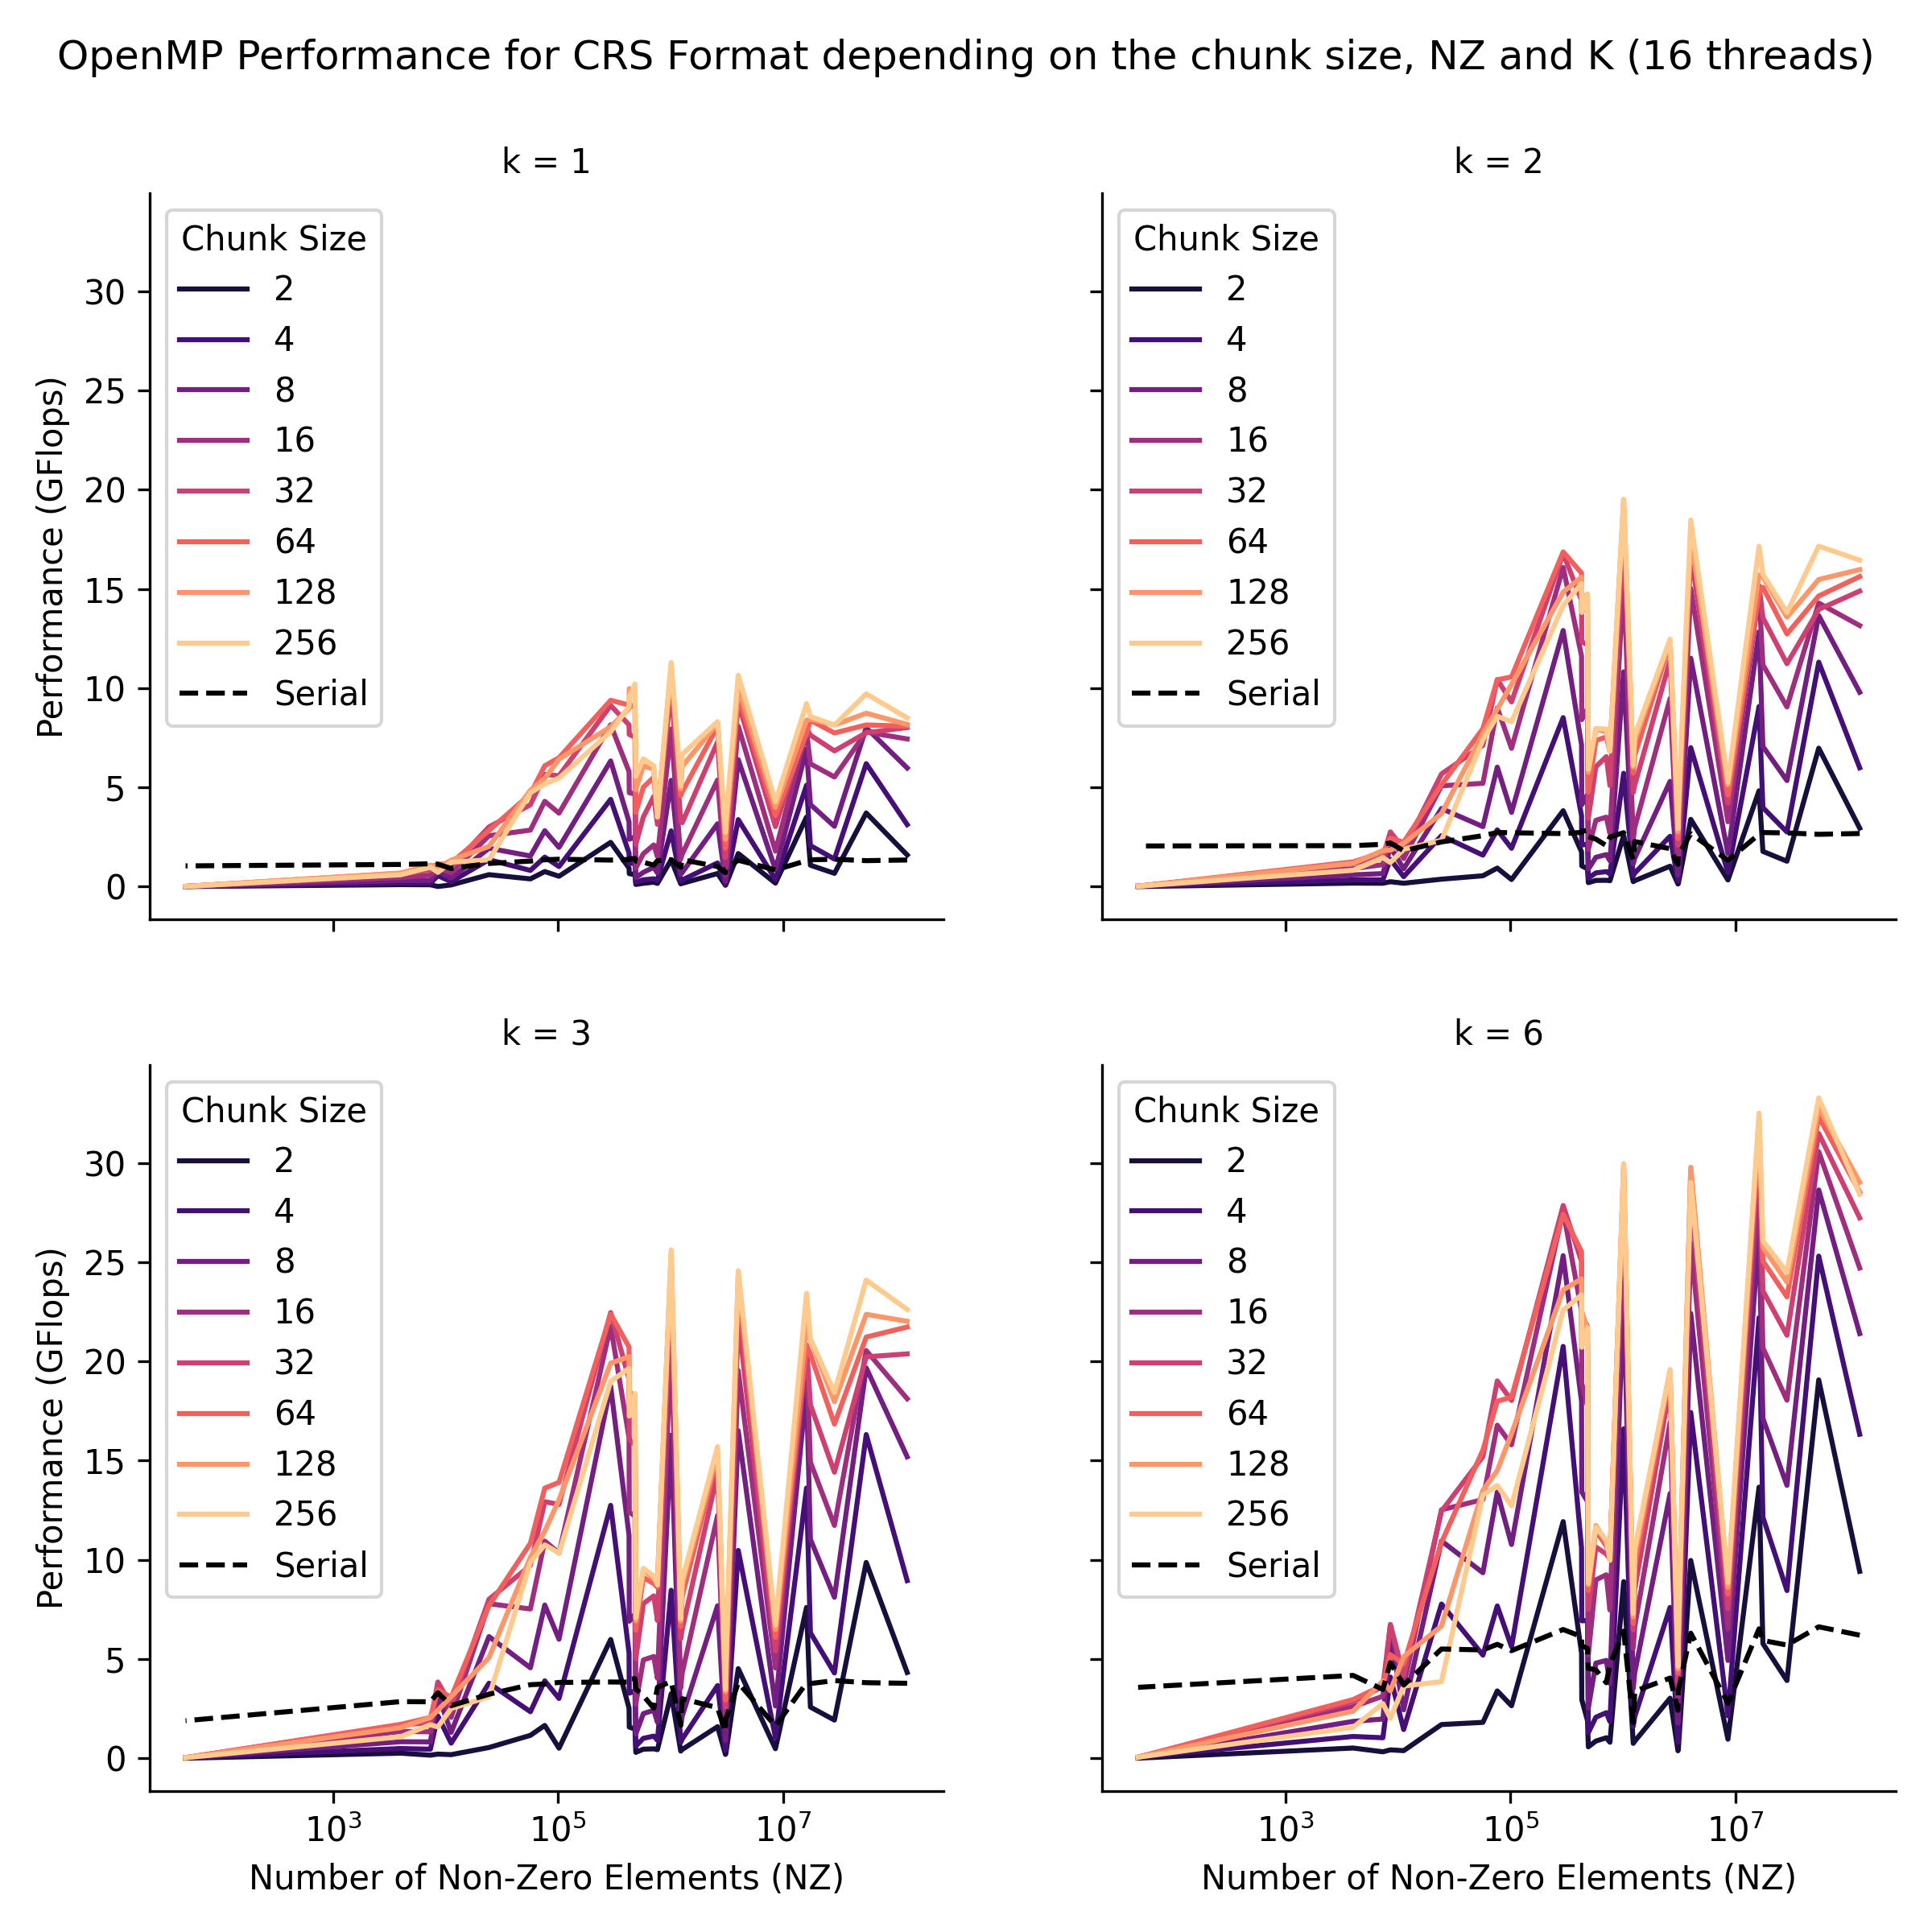
\includegraphics[width=0.6\textwidth]{../results/images/openMP_ChunkSize_CRS.png}
    \caption{OpenMP Performance for CRS Format depending on Chunk Size}
    \label{fig:openmpchunksizecrs}
\end{figure}

\begin{figure}[H]
    \centering
    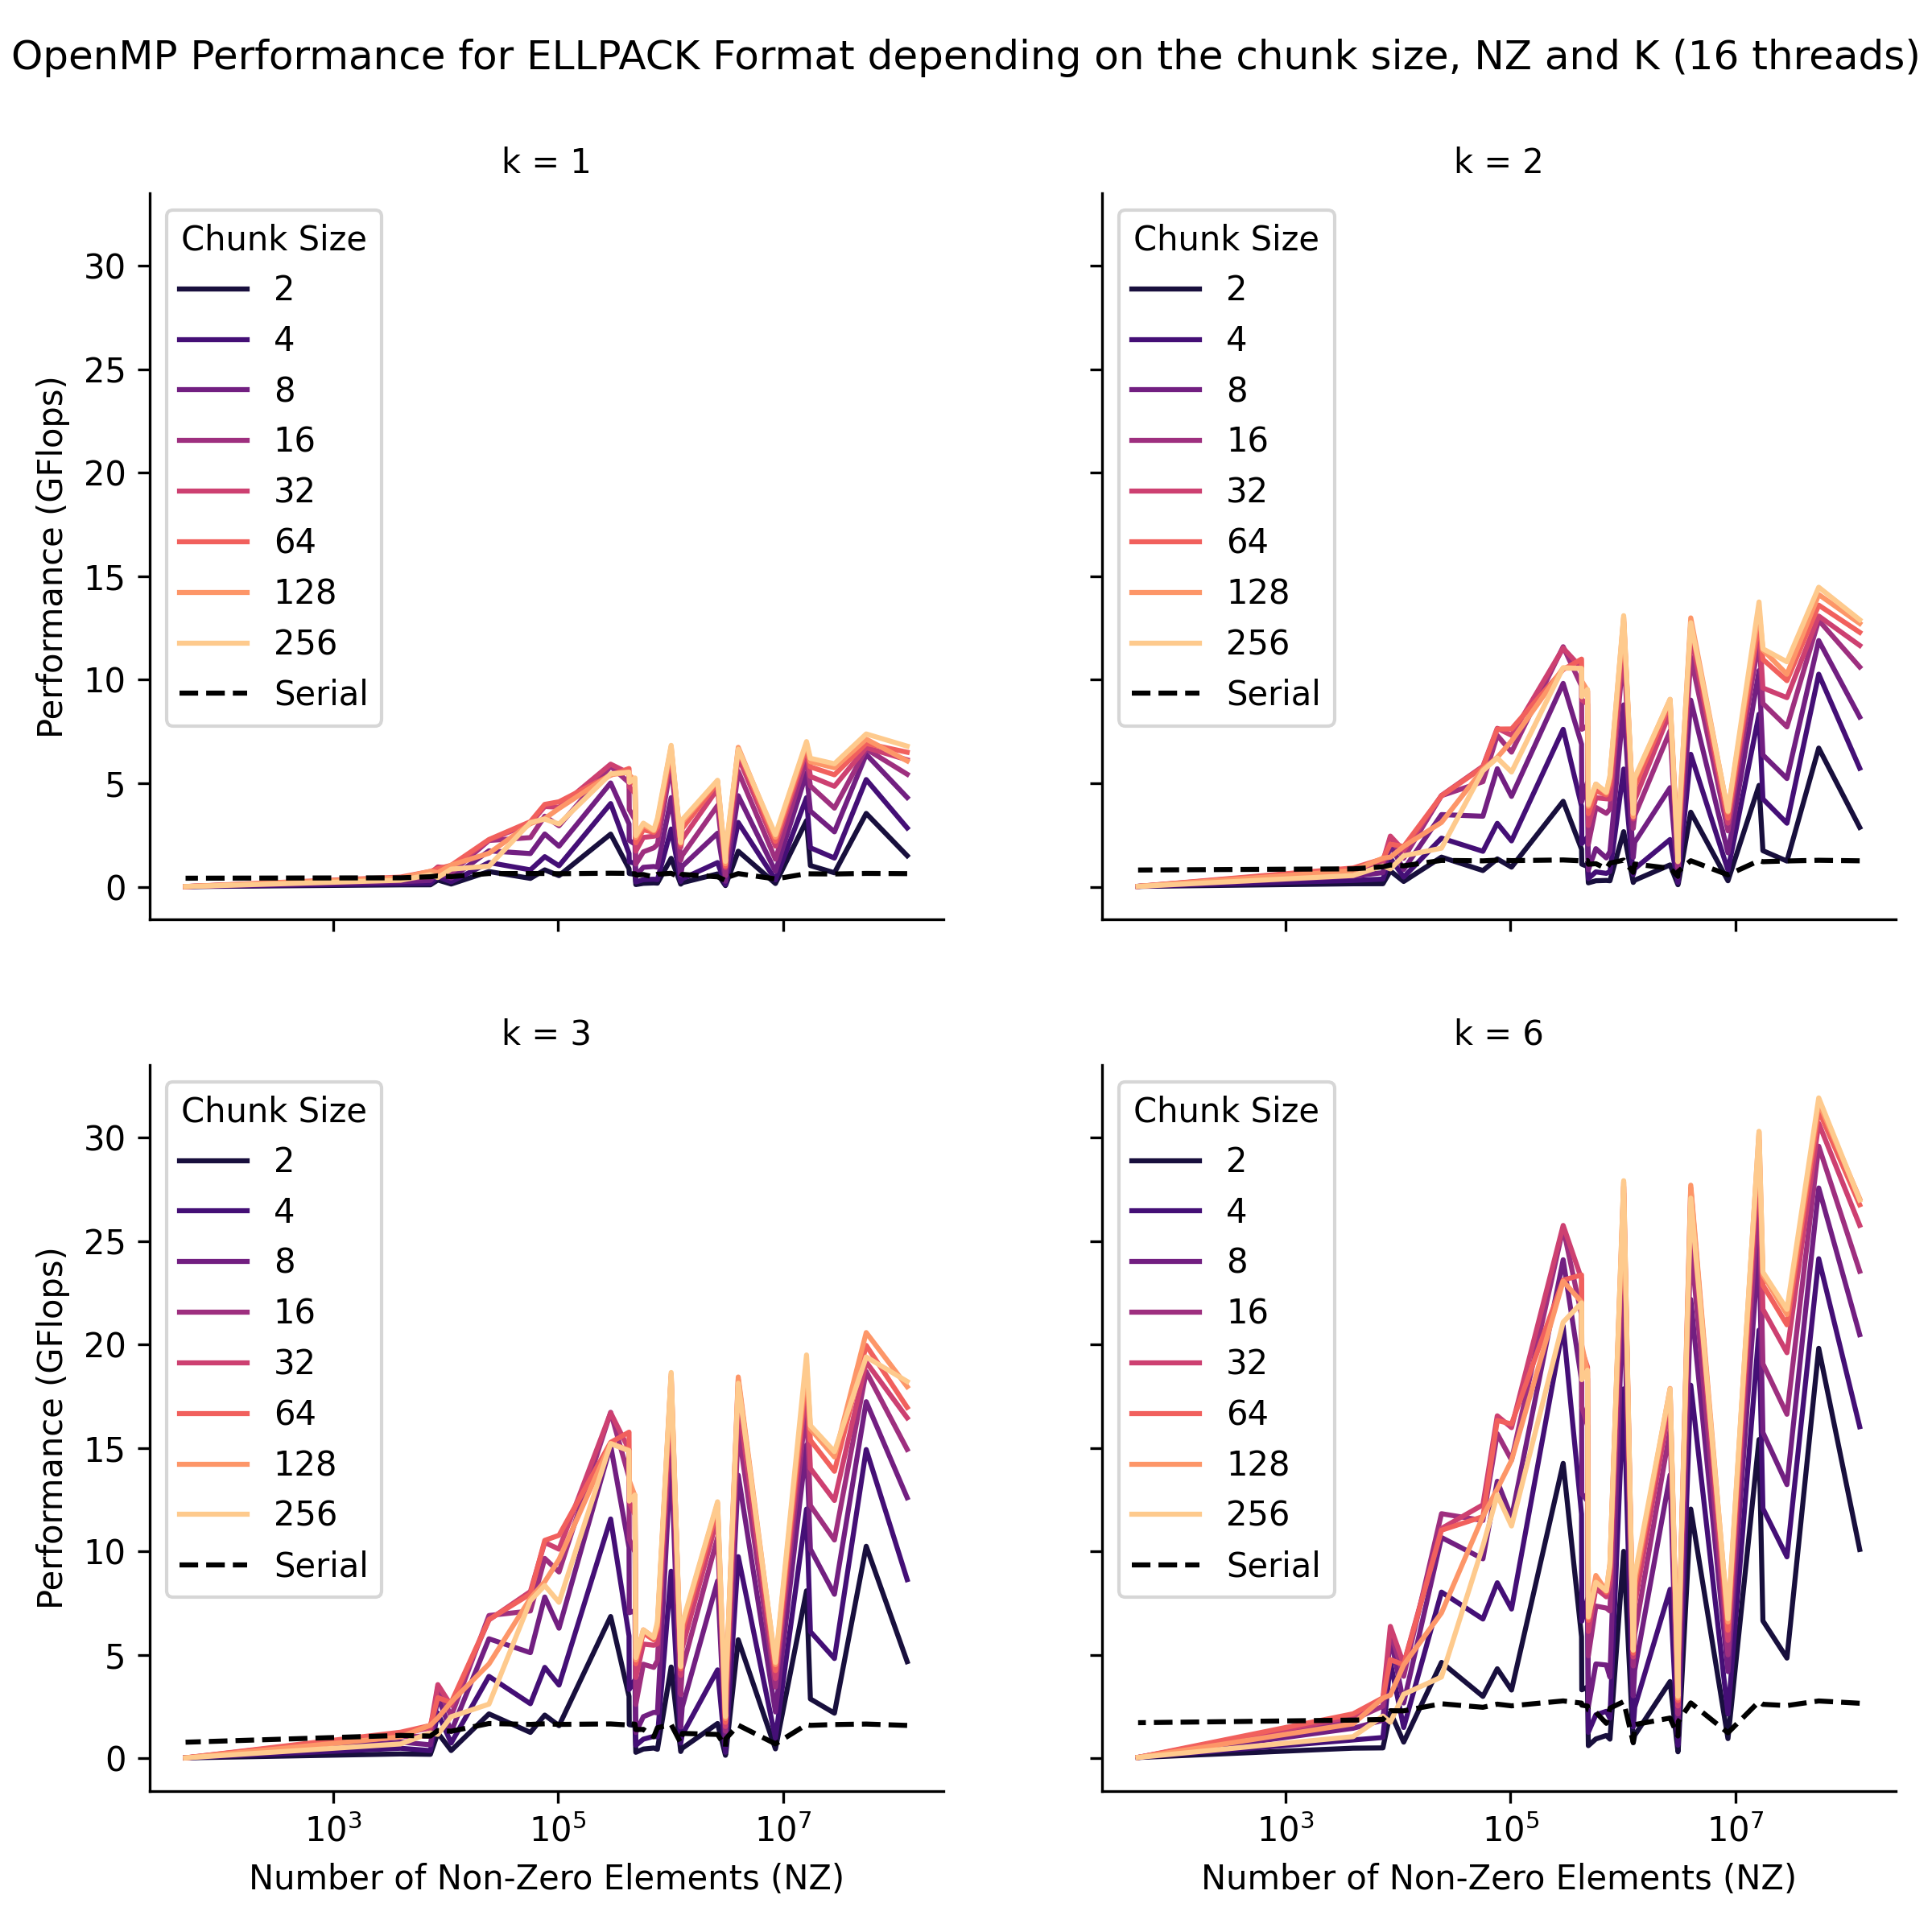
\includegraphics[width=0.6\textwidth]{../results/images/openMP_ChunkSize_ELLPACK.png}
    \caption{OpenMP Performance for ELLPACK Format depending on Chunk Size}
    \label{fig:openmpchunksizellpack}
\end{figure}

As shown in Figures~\ref{fig:openmpchunksizecrs} and
\ref{fig:openmpchunksizellpack}, the performance of the OpenMP parallel
algorithms is influenced by the chunk size. For lower sparsity matrices, the
optimal chunk size is 64 for the CRS format and 32 for the ELLPACK format. For
higher sparsity matrices, the optimal chunk size is 128 or 256 for both
formats.

\subsubsection{Thread Count Analysis}
\begin{figure}[H]
    \centering
    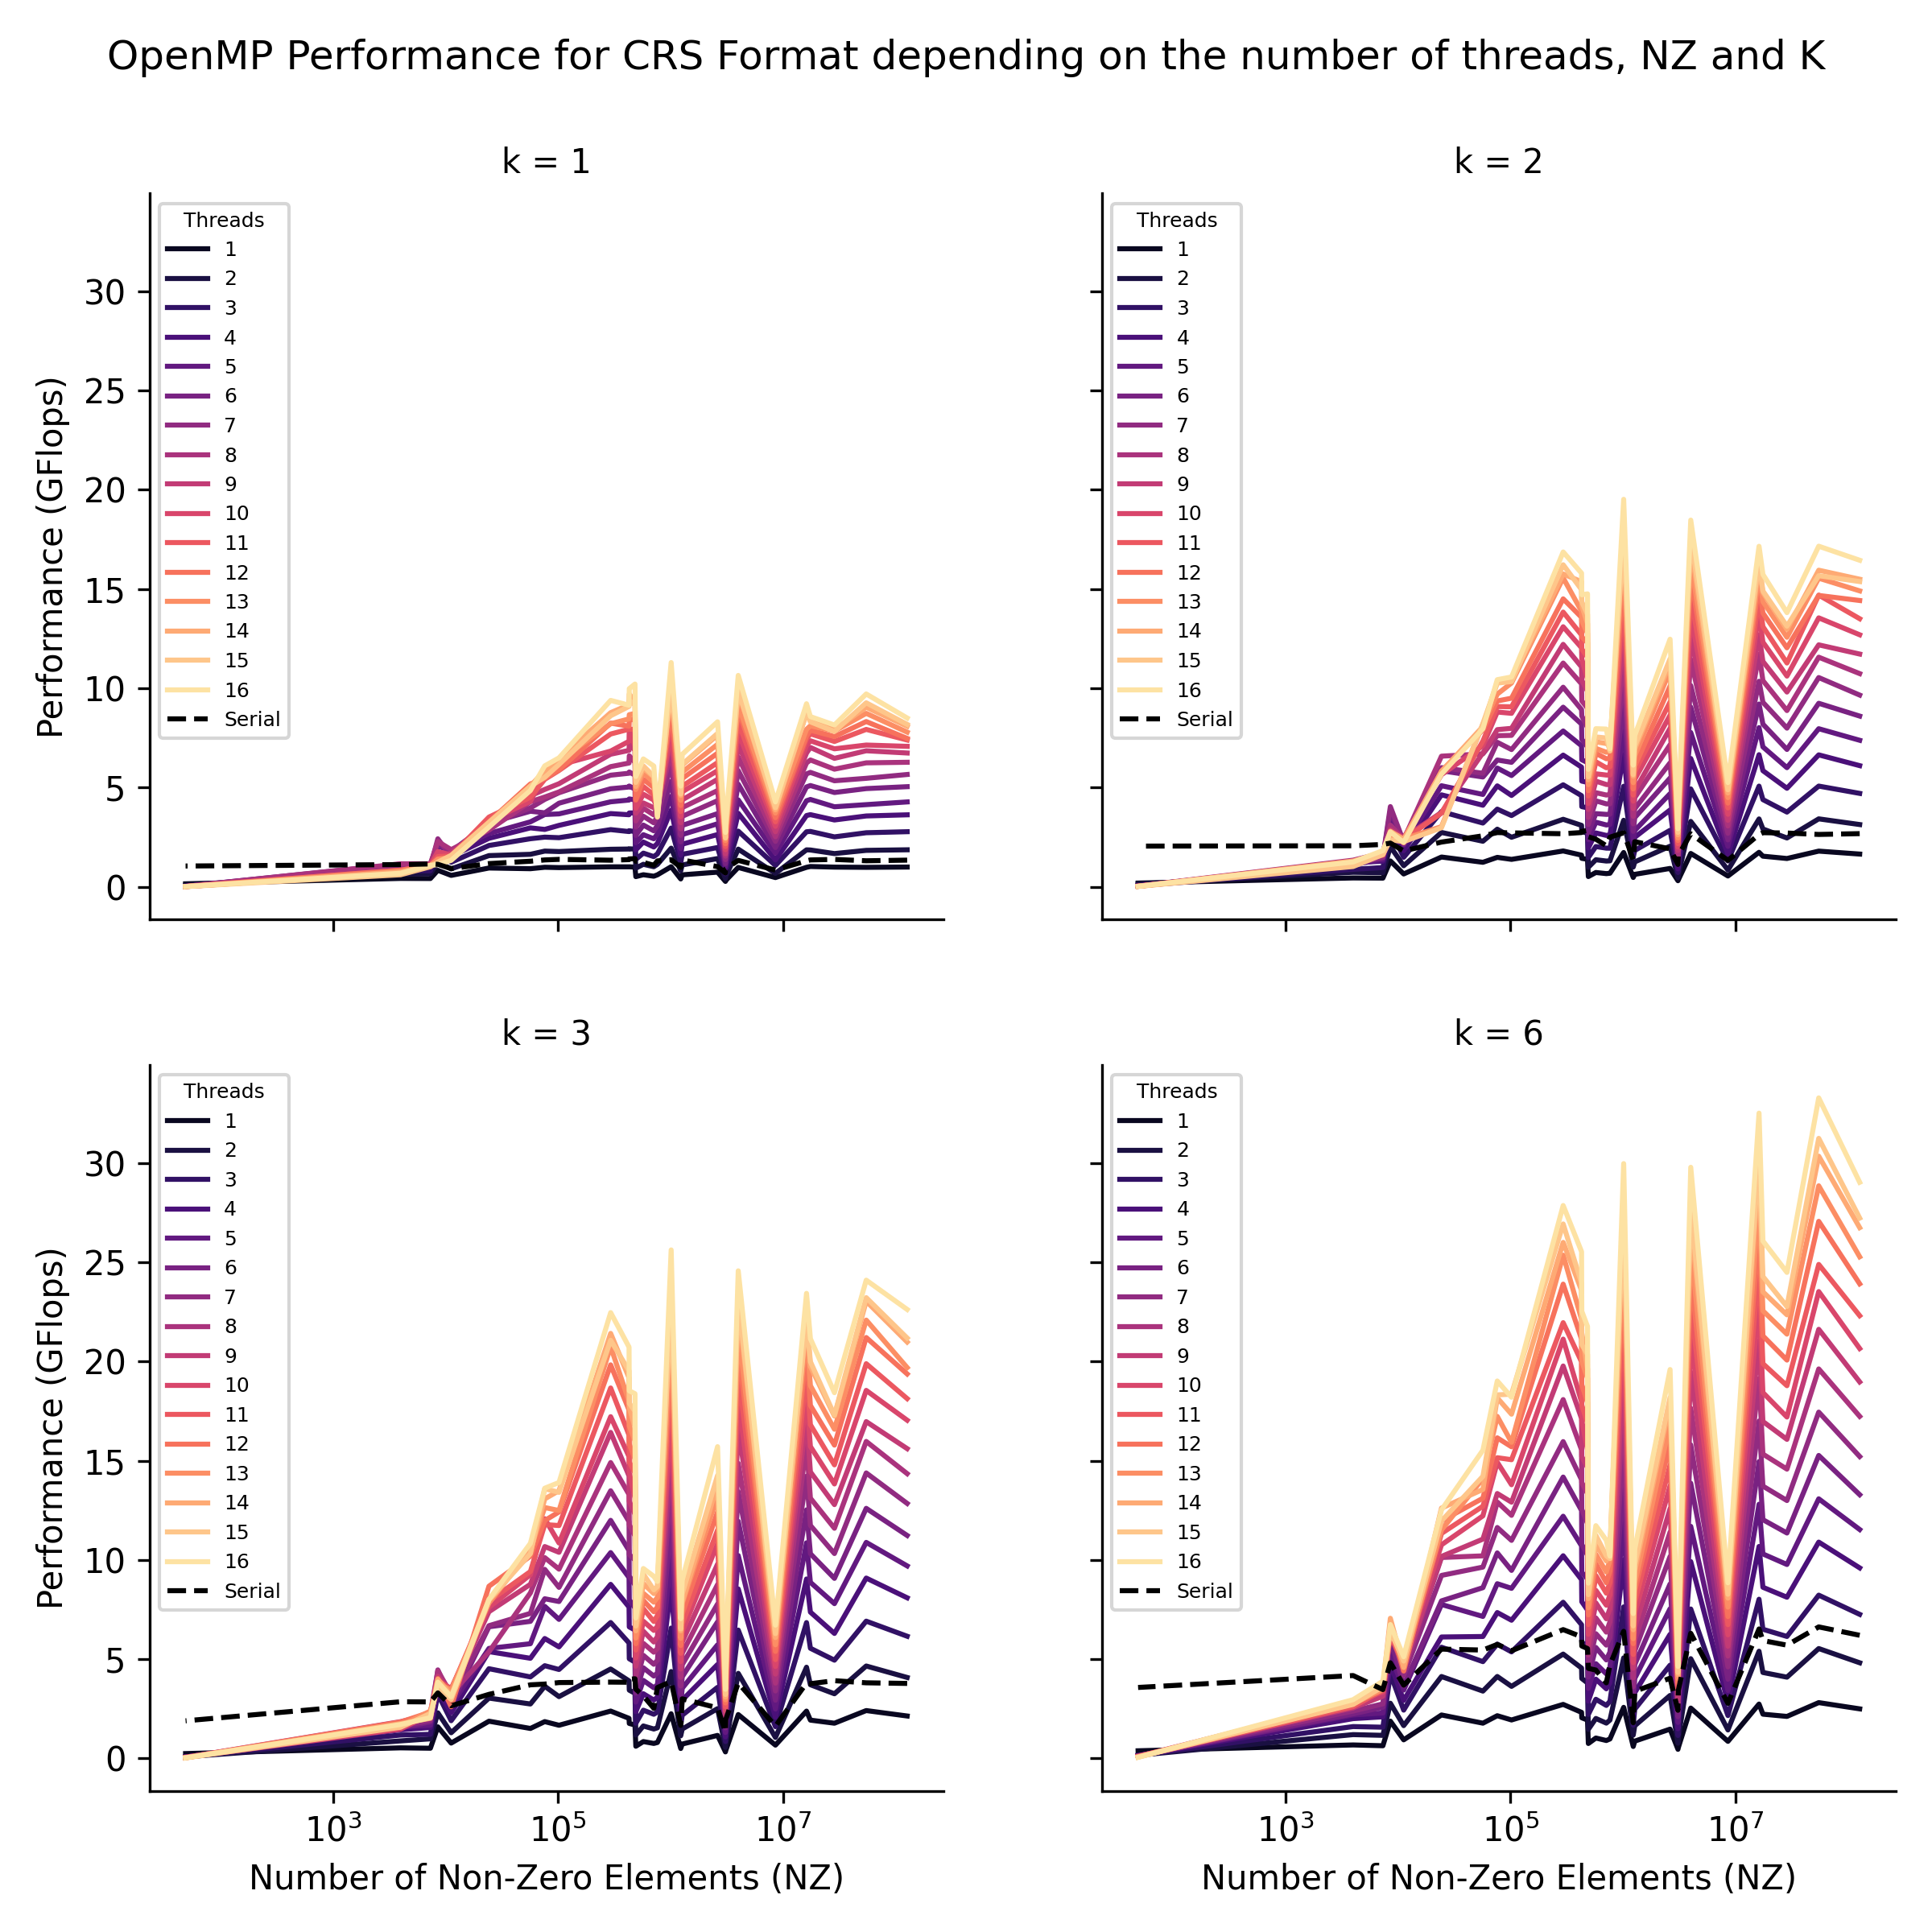
\includegraphics[width=0.6\textwidth]{../results/images/openMP_Threads_CRS.png}
    \caption{OpenMP Performance for CRS Format depending on Threads}
    \label{fig:openmpthreadscrs}
\end{figure}

\begin{figure}[H]
    \centering
    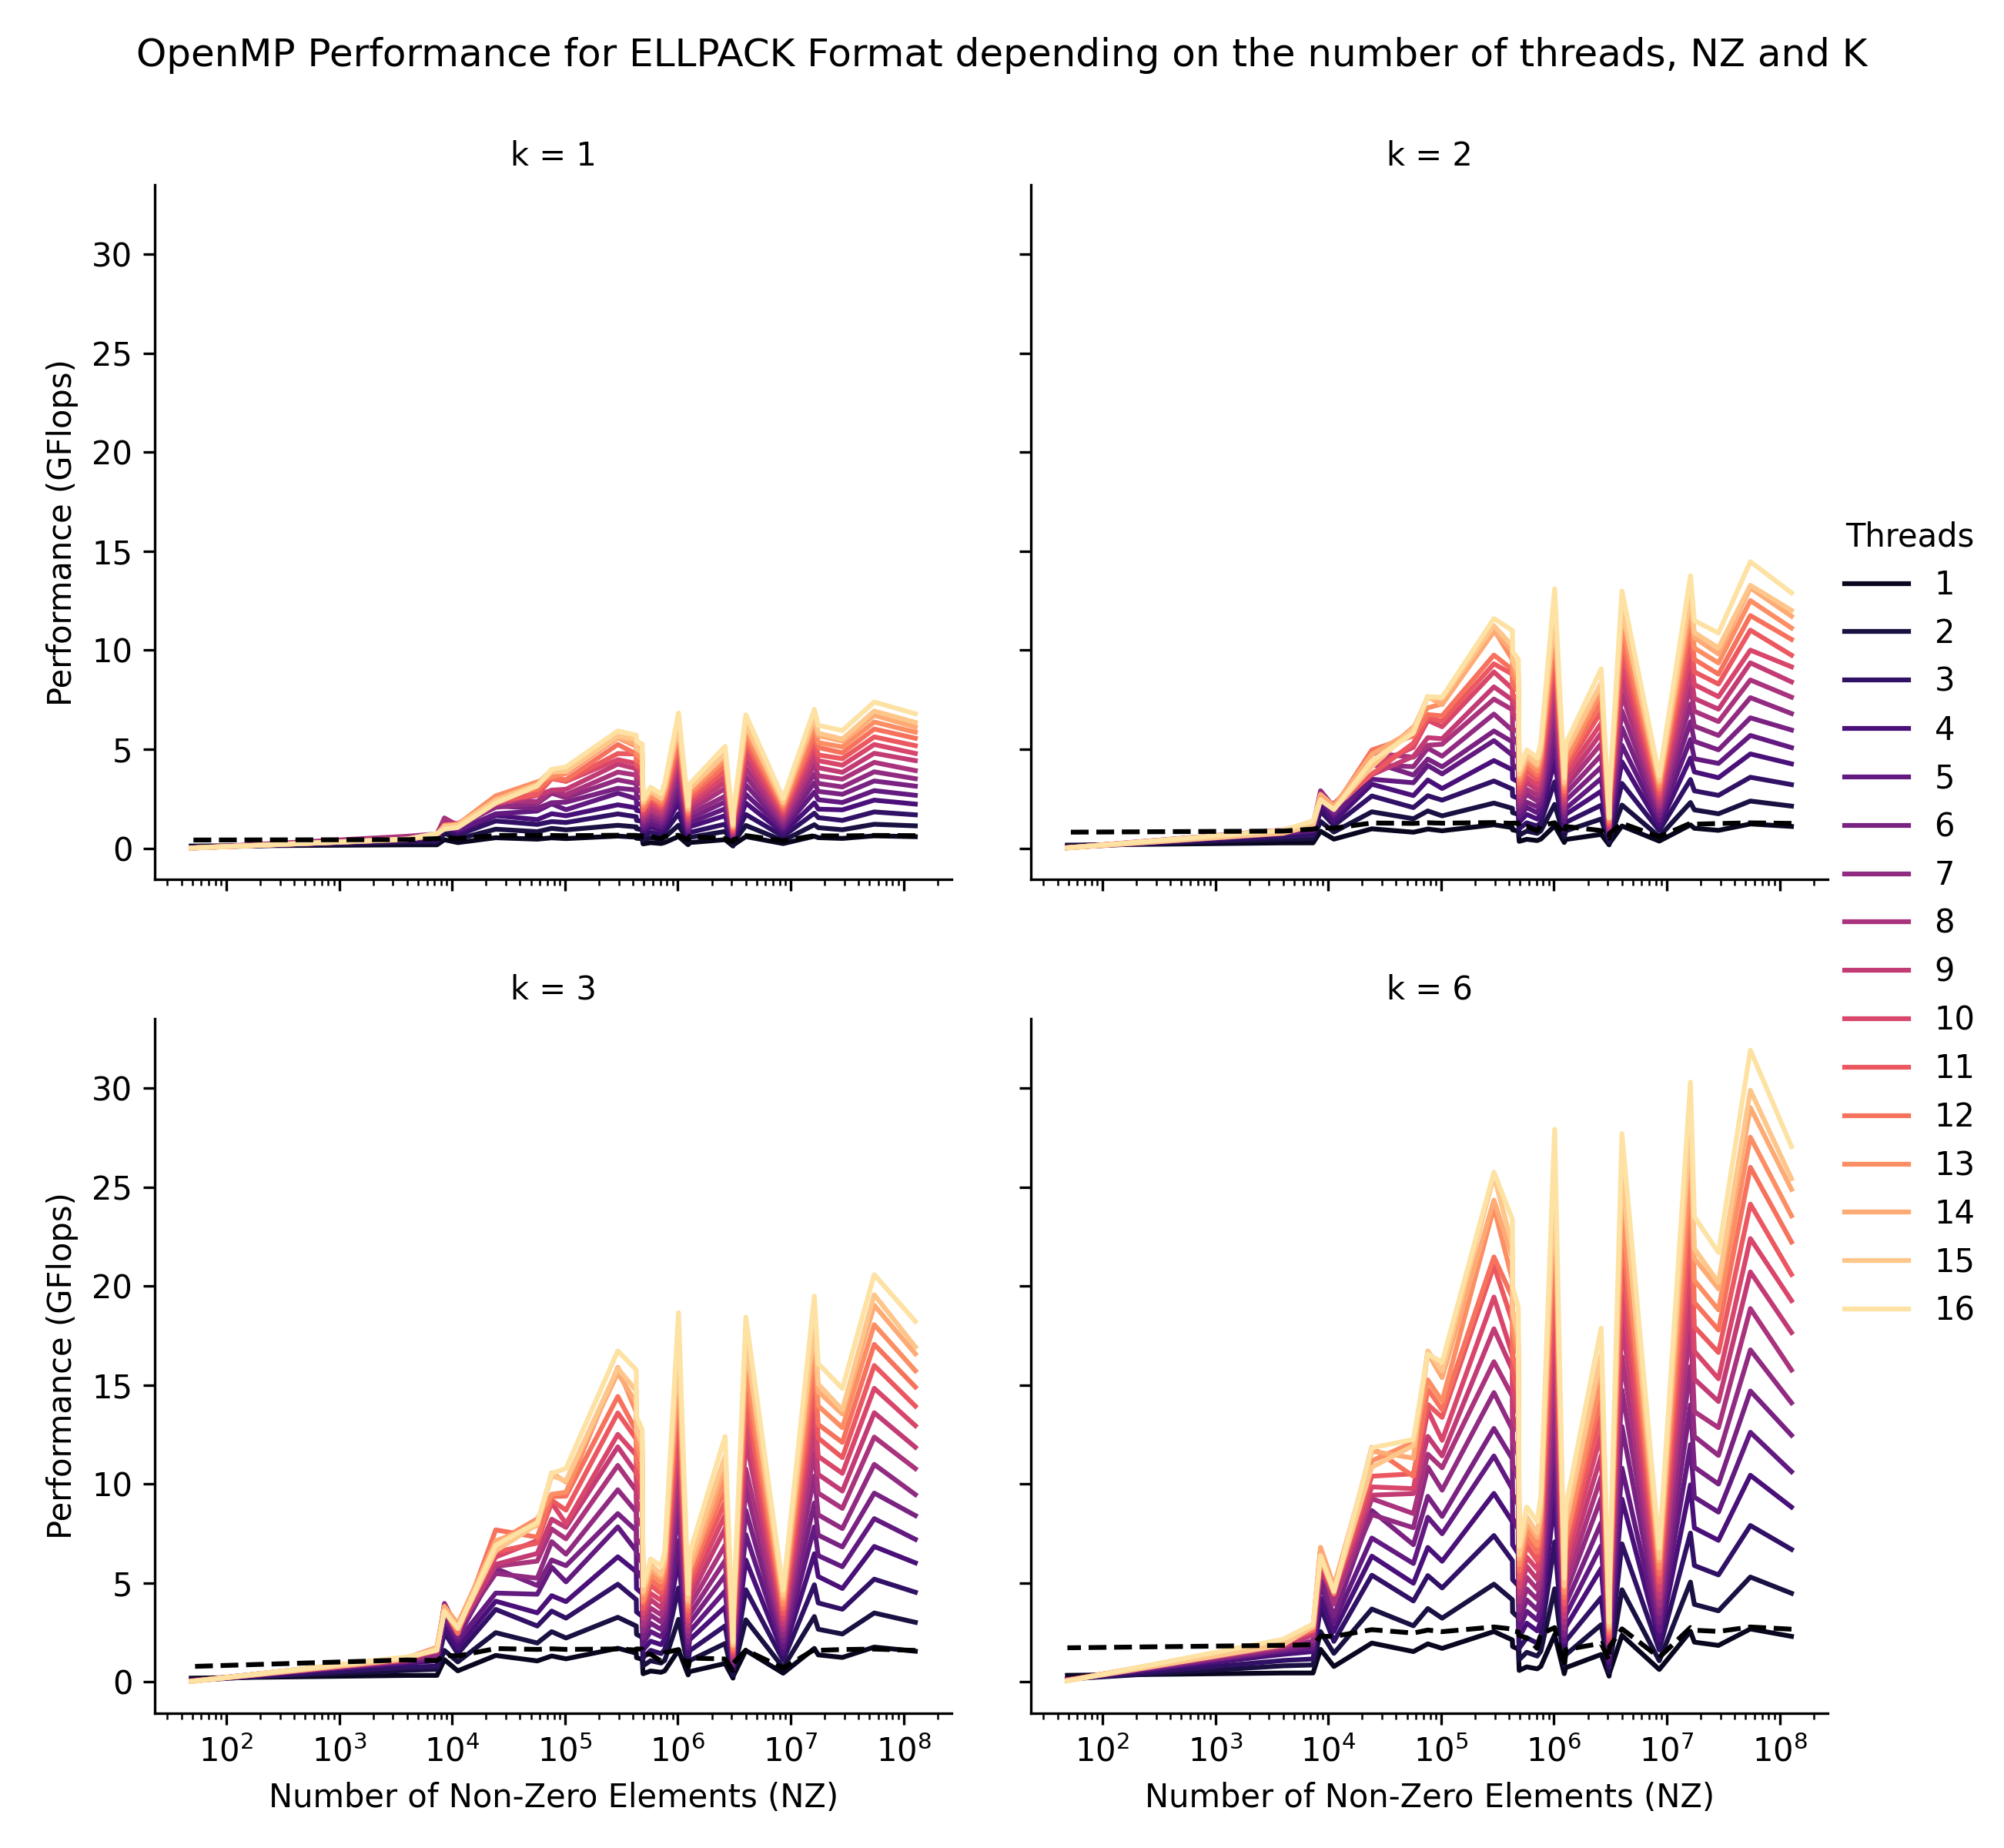
\includegraphics[width=0.6 \textwidth]{../results/images/openMP_Threads_ELLPACK.png}
    \caption{OpenMP Performance for ELLPACK Format depending on Threads}
    \label{fig:openmpthreadsellpack}
\end{figure}

As shown in Figures~\ref{fig:openmpthreadscrs} and
\ref{fig:openmpthreadsellpack}, the performance of the OpenMP parallel
algorithms is influenced by the number of threads. As more threads are used,
the performance improves up to a certain point, after which the performance
starts to stagnate due to the overhead of managing the threads.

\subsubsection{Performance Comparison}
\begin{figure}[H]
    \centering
    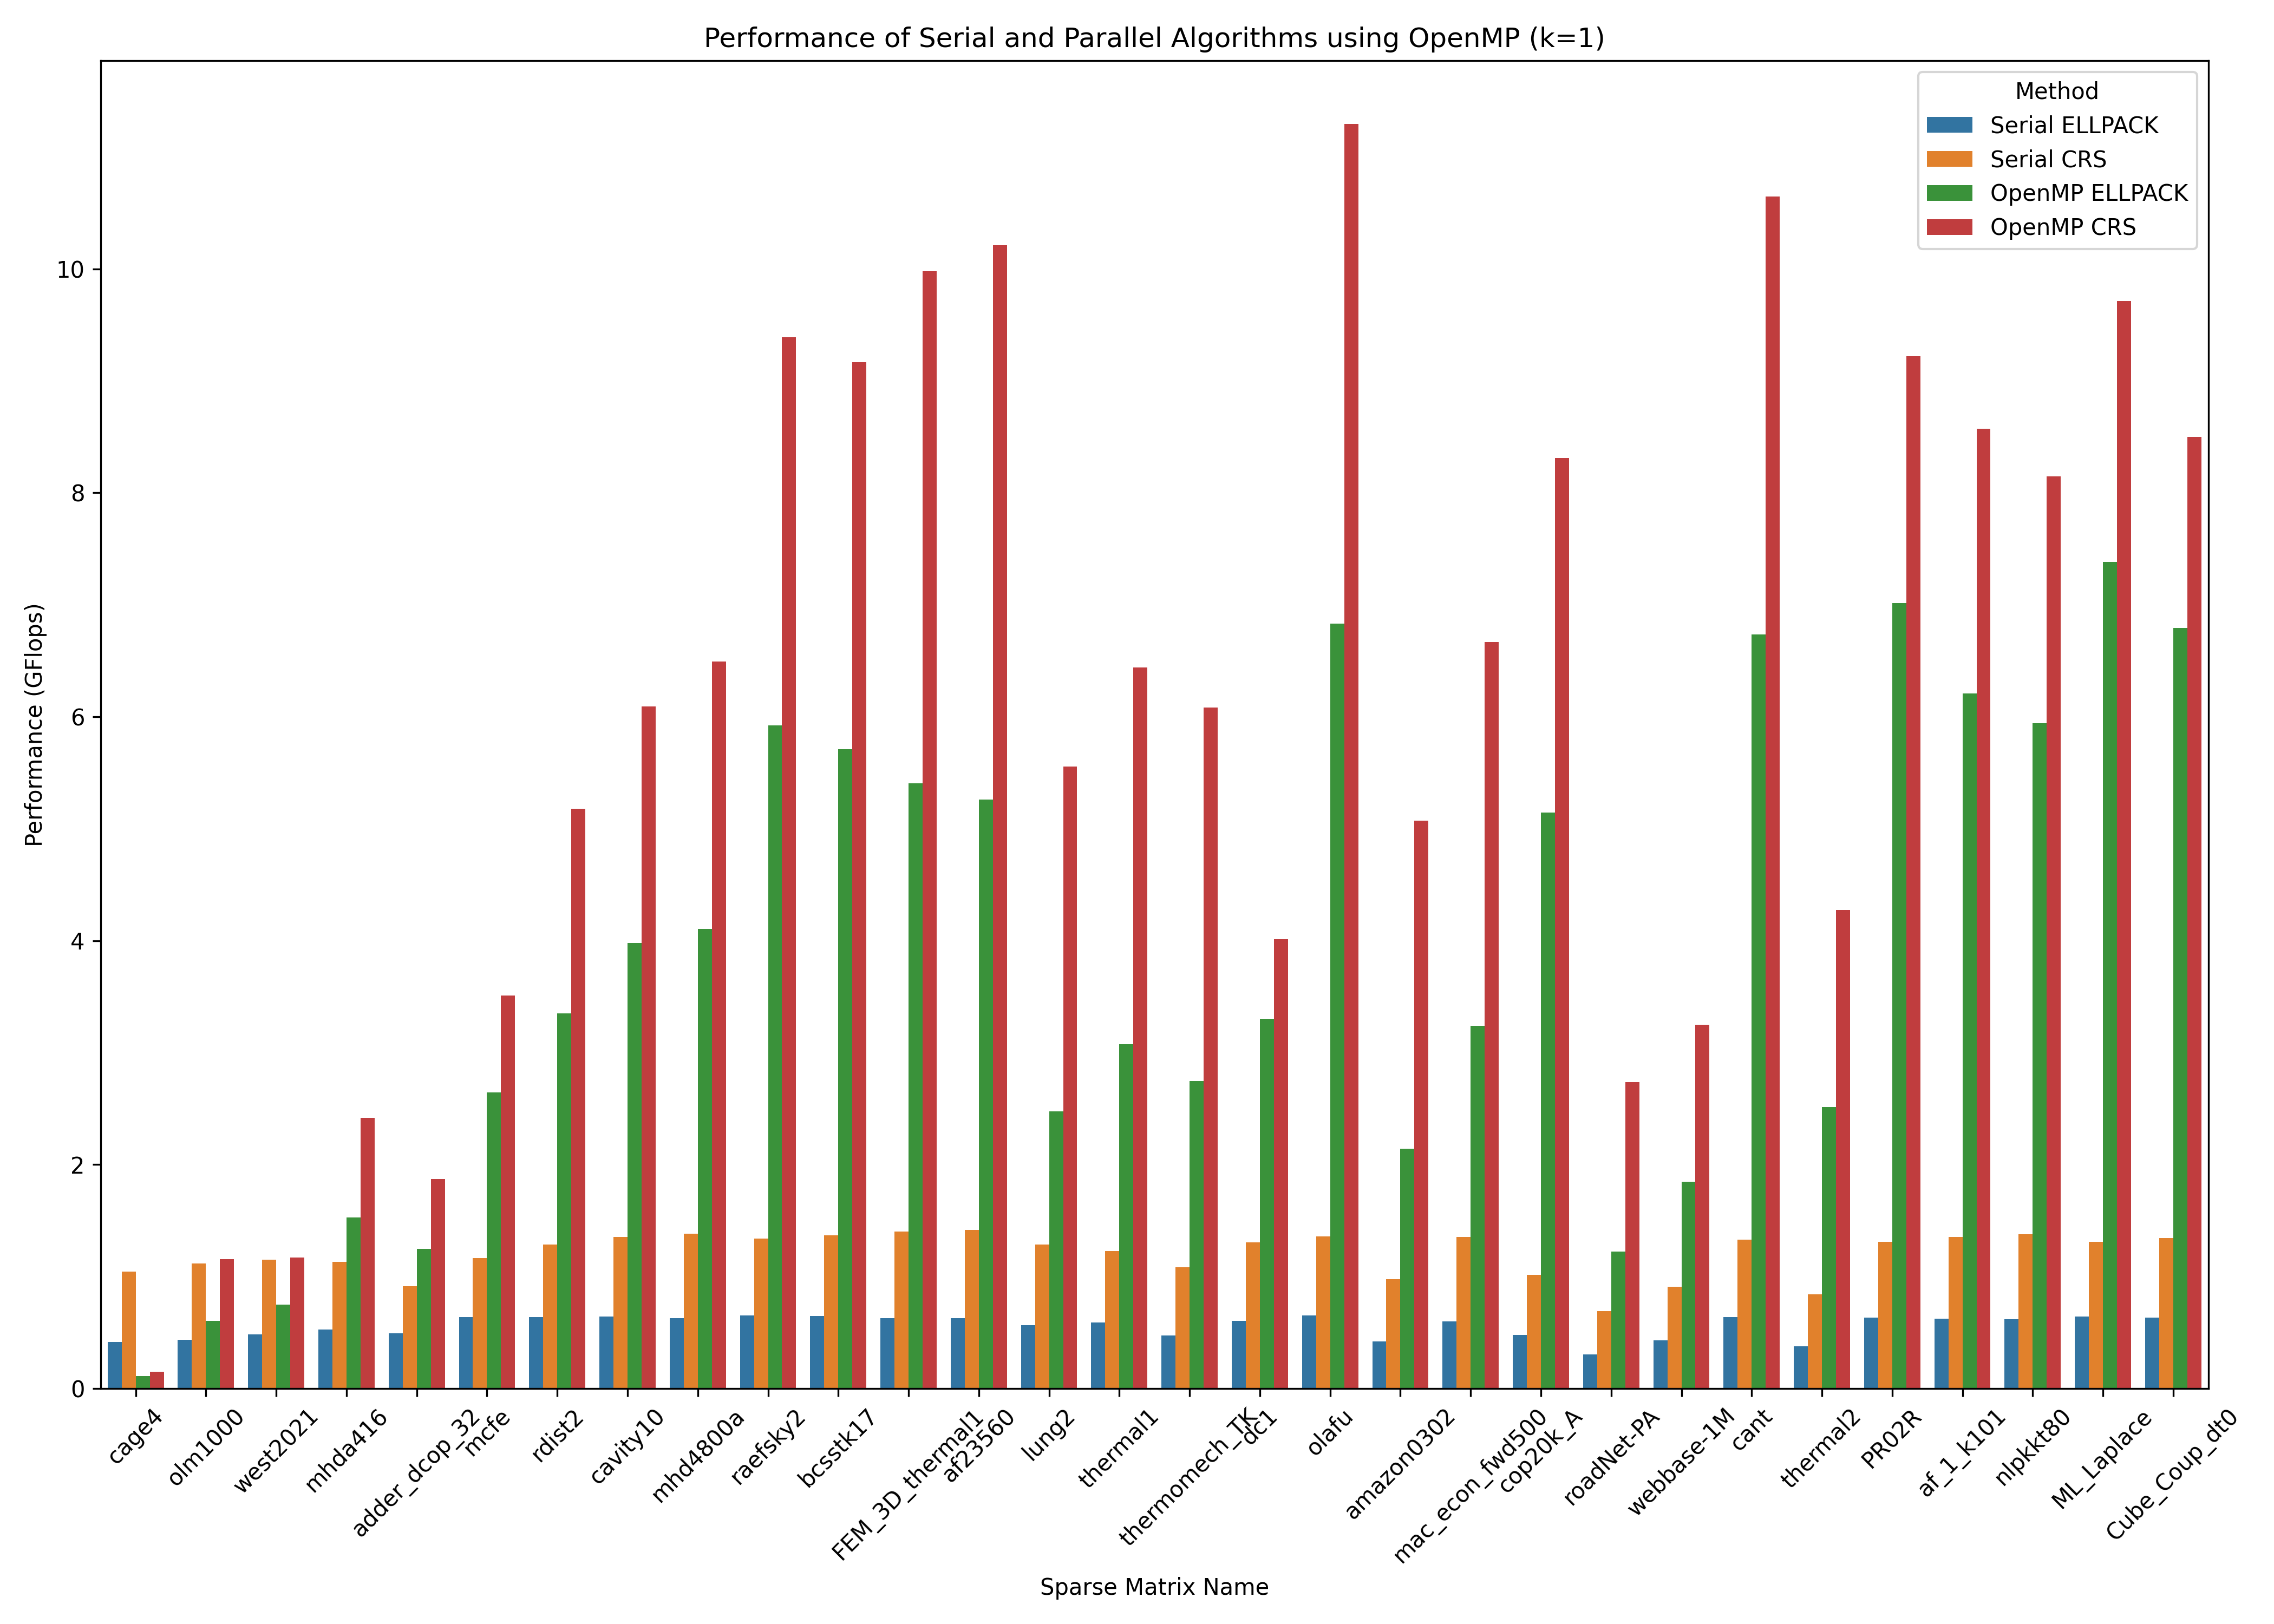
\includegraphics[width=0.9\textwidth]{../results/images/openMP_Performance_k1.png}
    \caption{Performance of Serial and Parallel Algorithms using OpenMP for $k=1$}
    \label{fig:openmp-performance-k1}
\end{figure}

\begin{figure}[H]
    \centering
    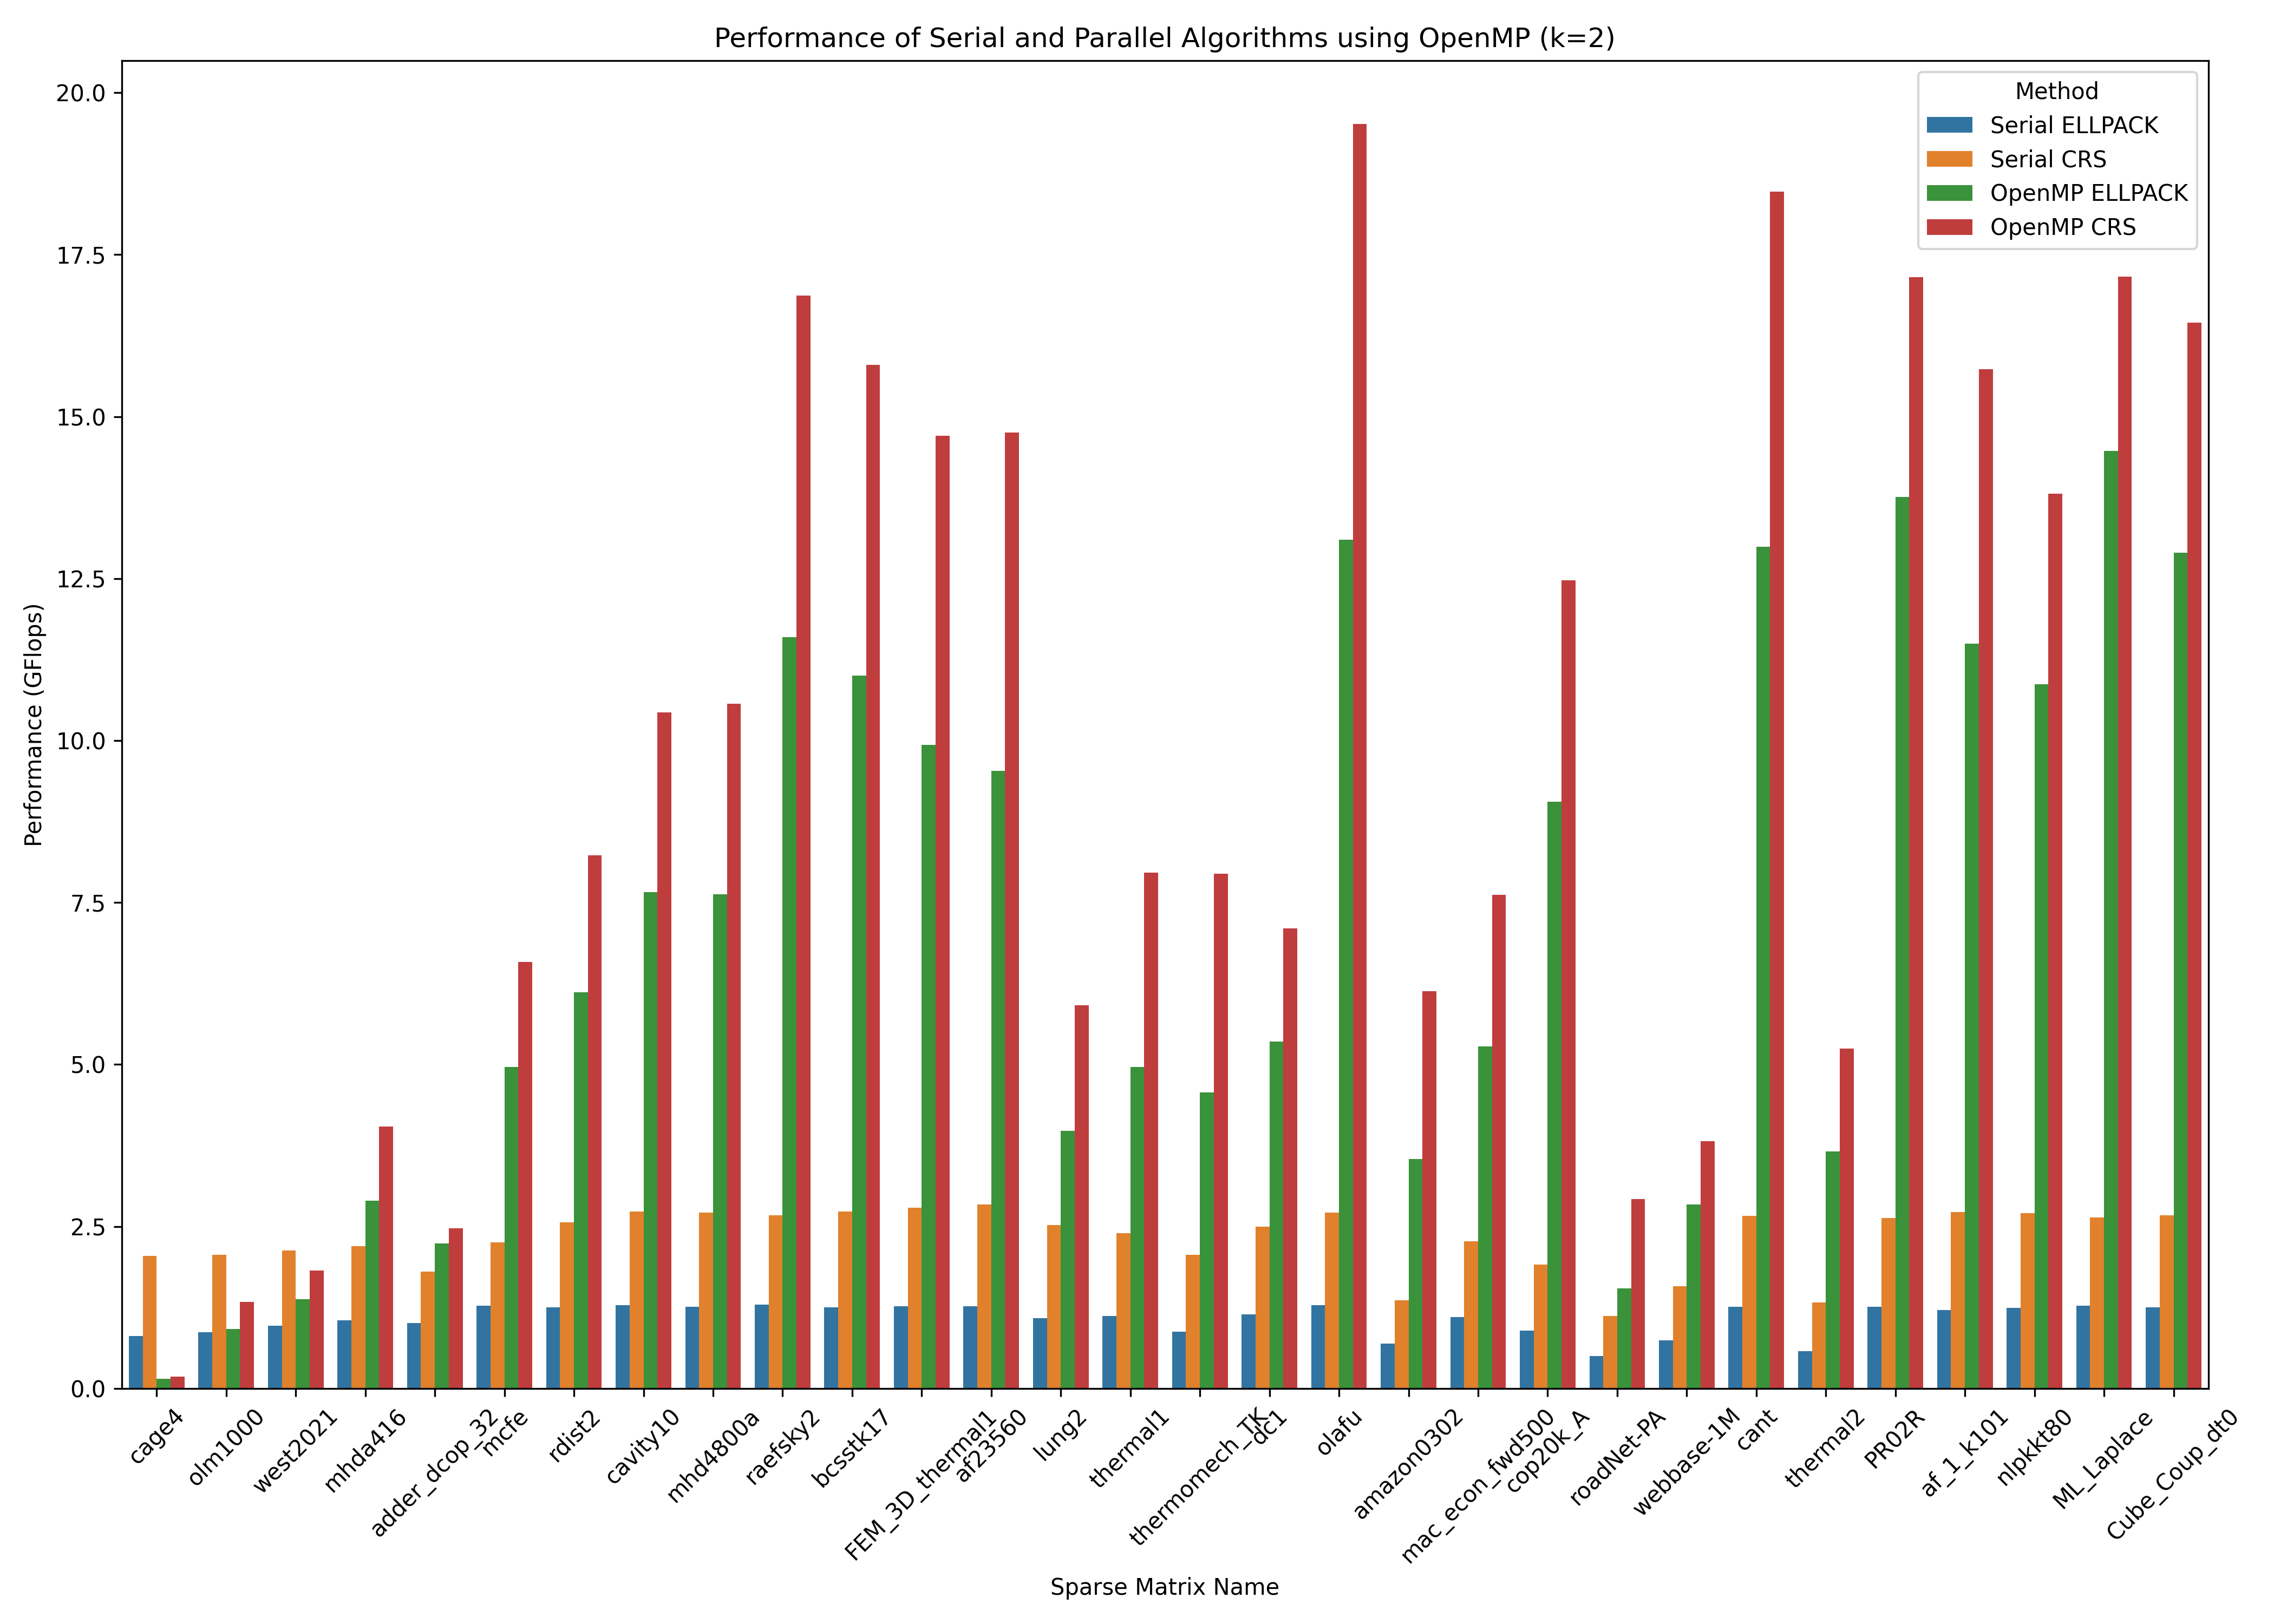
\includegraphics[width=0.9\textwidth]{../results/images/openMP_Performance_k2.png}
    \caption{Performance of Serial and Parallel Algorithms using OpenMP for $k=2$}
    \label{fig:openmp-performance-k2}
\end{figure}

\begin{figure}[H]
    \centering
    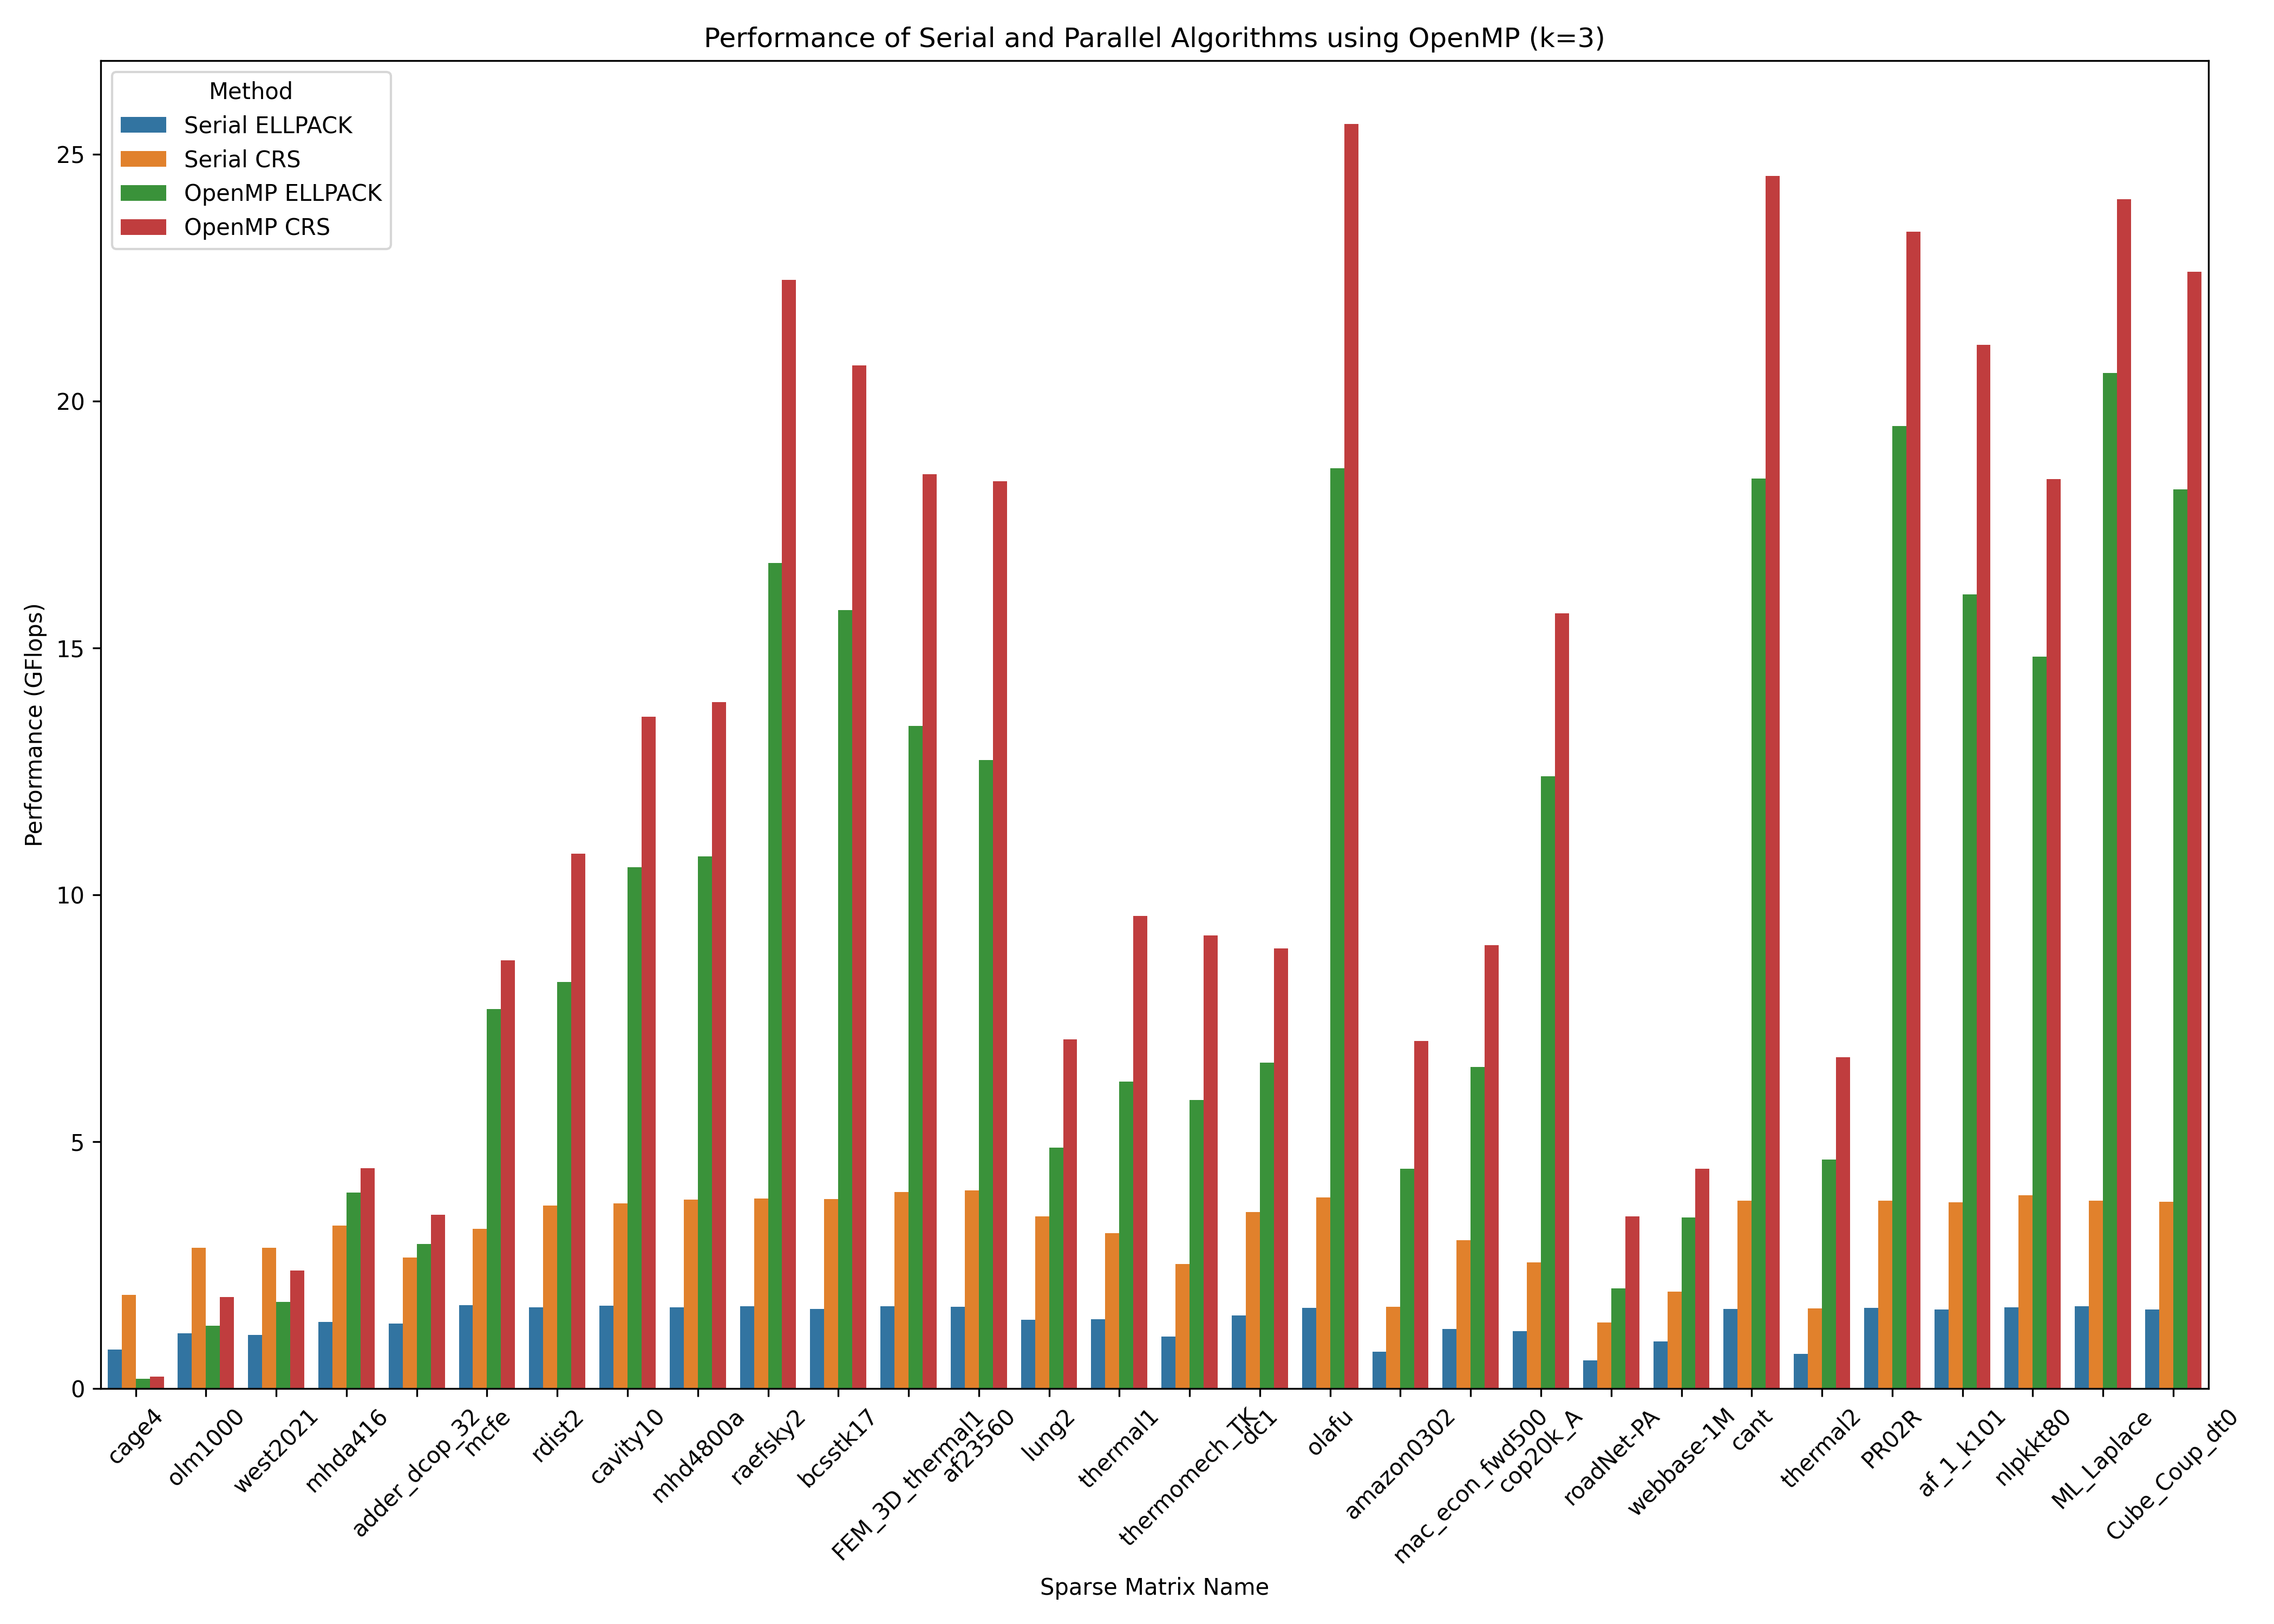
\includegraphics[width=0.9\textwidth]{../results/images/openMP_Performance_k3.png}
    \caption{Performance of Serial and Parallel Algorithms using OpenMP for $k=3$}
    \label{fig:openmp-performance-k3}
\end{figure}

\begin{figure}[H]
    \centering
    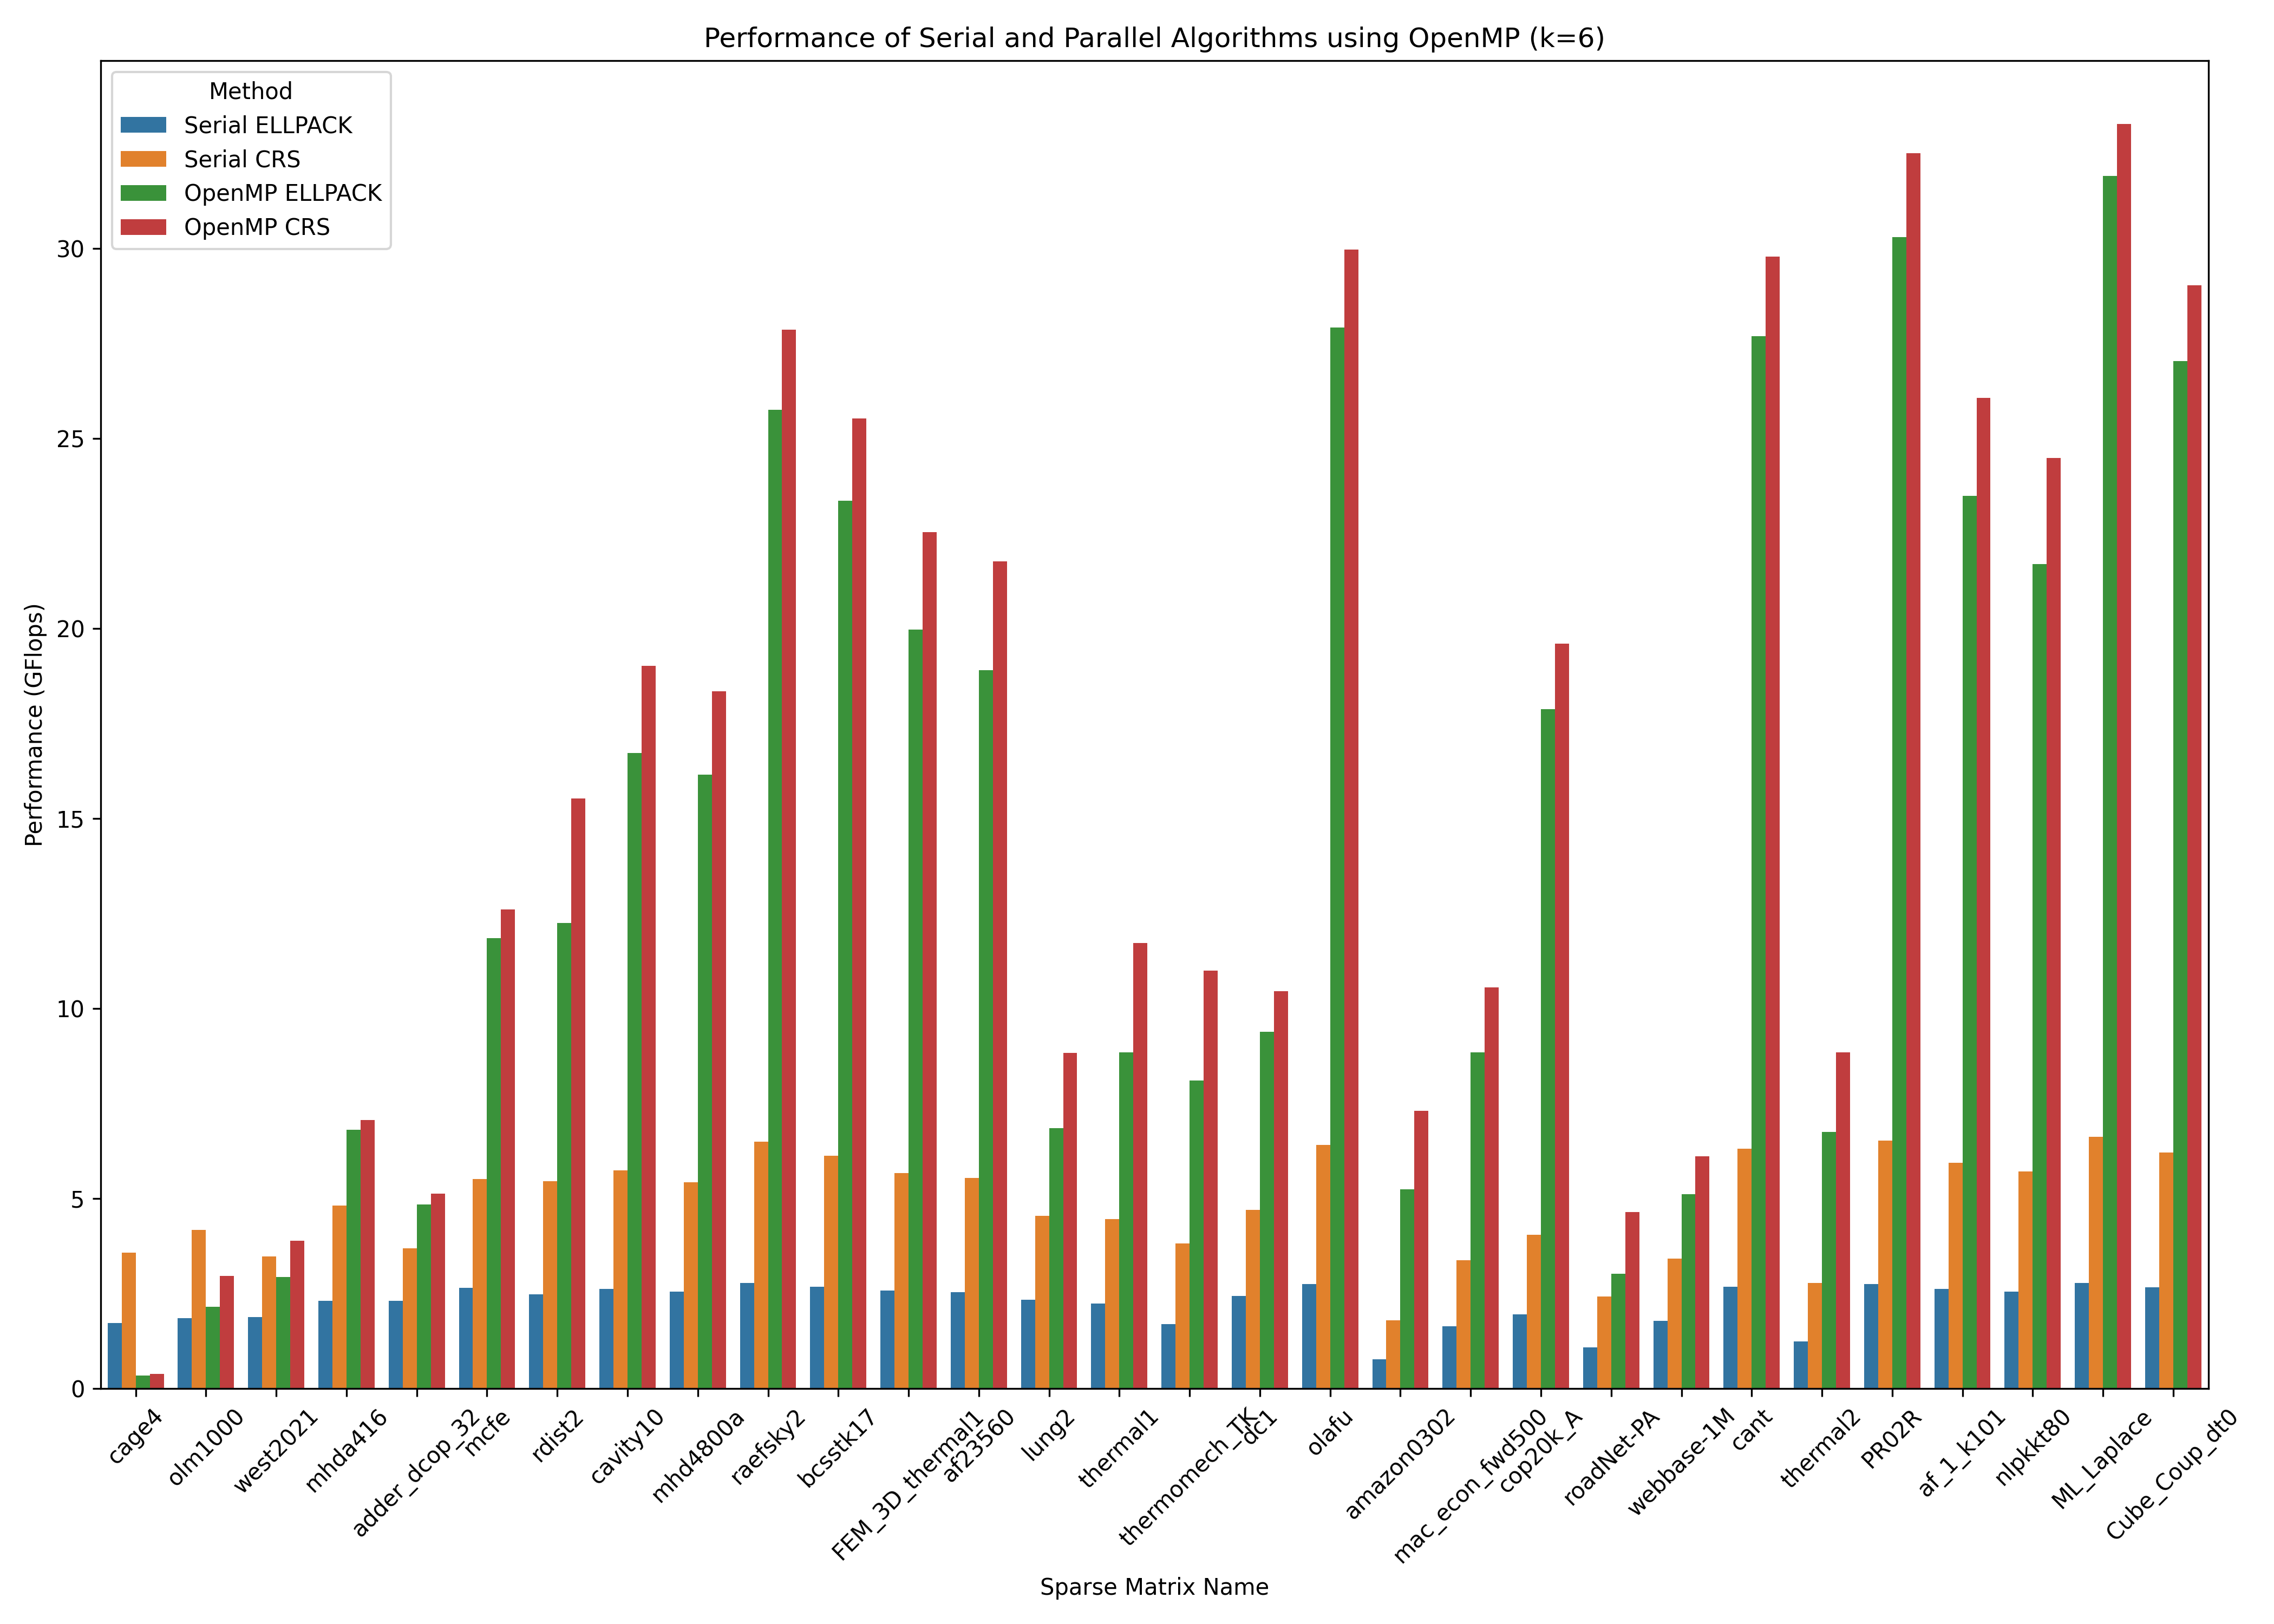
\includegraphics[width=0.9\textwidth]{../results/images/openMP_Performance_k6.png}
    \caption{Performance of Serial and Parallel Algorithms using OpenMP for $k=6$}
    \label{fig:openmp-performance-k6}
\end{figure}

As shown in Figures~\ref{fig:openmp-performance-k1},

%TC:ignore 
\begin{longtable}{lcccr}
    \caption{CRS vs ELLPACK using OpenMP}                                                            \\
    \label{tab:crsvsellpackopenmp}                                                                   \\
    \toprule
    \textbf{Matrix}   & \textbf{CRS} & \textbf{ELLPACK} & \textbf{Best Structure} & \textbf{Speedup} \\
    \midrule
    \endfirsthead
    \toprule
    \textbf{Matrix}   & \textbf{CRS} & \textbf{ELLPACK} & \textbf{Best Structure} & \textbf{Speedup} \\
    \midrule
    \endhead
    \bottomrule
    \endfoot
    Cube\_Coup\_dt0   & 29.0243      & 27.0415          & CRS                     & 4.597152         \\
    FEM\_3D\_thermal1 & 22.5277      & 19.9711          & CRS                     & 3.792766         \\
    ML\_Laplace       & 33.2766      & 31.9121          & CRS                     & 5.019799         \\
    PR02R             & 32.5086      & 30.2968          & CRS                     & 4.942094         \\
    adder\_dcop\_32   & 5.12204      & 4.83417          & CRS                     & 1.142991         \\
    af23560           & 21.7606      & 18.9078          & CRS                     & 3.748958         \\
    af\_1\_k101       & 26.067       & 23.4946          & CRS                     & 4.245709         \\
    amazon0302        & 7.29883      & 5.23835          & CRS                     & 3.113809         \\
    bcsstk17          & 25.5293      & 23.3597          & CRS                     & 4.080255         \\
    cage4             & 0.385164     & 0.334653         & CRS                     & 0.441890         \\
    cant              & 29.7794      & 27.6956          & CRS                     & 4.638745         \\
    cavity10          & 19.0148      & 16.7258          & CRS                     & 3.152232         \\
    cop20k\_A         & 19.5918      & 17.8729          & CRS                     & 4.105772         \\
    dc1               & 10.4524      & 9.39085          & CRS                     & 2.230150         \\
    lung2             & 8.832        & 6.85328          & CRS                     & 1.905592         \\
    mac\_econ\_fwd500 & 10.5515      & 8.84879          & CRS                     & 2.863691         \\
    mcfe              & 12.6097      & 11.8456          & CRS                     & 2.077682         \\
    mhd4800a          & 18.3501      & 16.1582          & CRS                     & 3.352021         \\
    mhda416           & 7.06099      & 6.80262          & CRS                     & 1.278130         \\
    nlpkkt80          & 24.4853      & 21.694           & CRS                     & 4.127566         \\
    olafu             & 29.966       & 27.9111          & CRS                     & 4.623662         \\
    olm1000           & 2.95895      & 2.1558           & CRS                     & 0.619634         \\
    raefsky2          & 27.8548      & 25.7504          & CRS                     & 4.248730         \\
    rdist2            & 15.5283      & 12.2527          & CRS                     & 2.694487         \\
    roadNet-PA        & 4.63584      & 3.01227          & CRS                     & 1.703601         \\
    thermal1          & 11.7254      & 8.83925          & CRS                     & 2.549122         \\
    thermal2          & 8.84723      & 6.75174          & CRS                     & 2.758931         \\
    thermomech\_TK    & 10.9908      & 8.10205          & CRS                     & 3.088284         \\
    webbase-1M        & 6.11469      & 5.10783          & CRS                     & 1.630393         \\
    west2021          & 3.89256      & 2.92762          & CRS                     & 0.930255         \\                                                                               \\
\end{longtable}
%TC:endignore

The performance evaluation of the CRS and ELLPACK formats, when parallelized
with OpenMP, shows a preference for CRS in a majority of cases. This trend,
indicated by a frequent superiority of the CRS format, highlights its
suitability for OpenMP's parallelization capabilities, probably due to more
optimal memory management and task distribution between threads.

The observed speed-up factor varies significantly between matrices, with
particularly remarkable speed-ups for matrices such as \textit{Cube\_Coup\_dt0}
and \textit{FEM\_3D\_thermal1}, highlighting the potential for improving
performance via OpenMP's parallel optimisation.

Special cases such as \textit{cage4} and \textit{olm1000} show lower speed-ups,
revealing the limits of parallelization for certain matrix structures. The
influence of matrix density and size is also notable, with high densities and
large dense vectors favouring the CRS format more, illustrating its
effectiveness in processing large workloads under OpenMP.

\subsection{CUDA}

\subsubsection{X Block Size Analysis}

\begin{figure}[H]
    \centering
    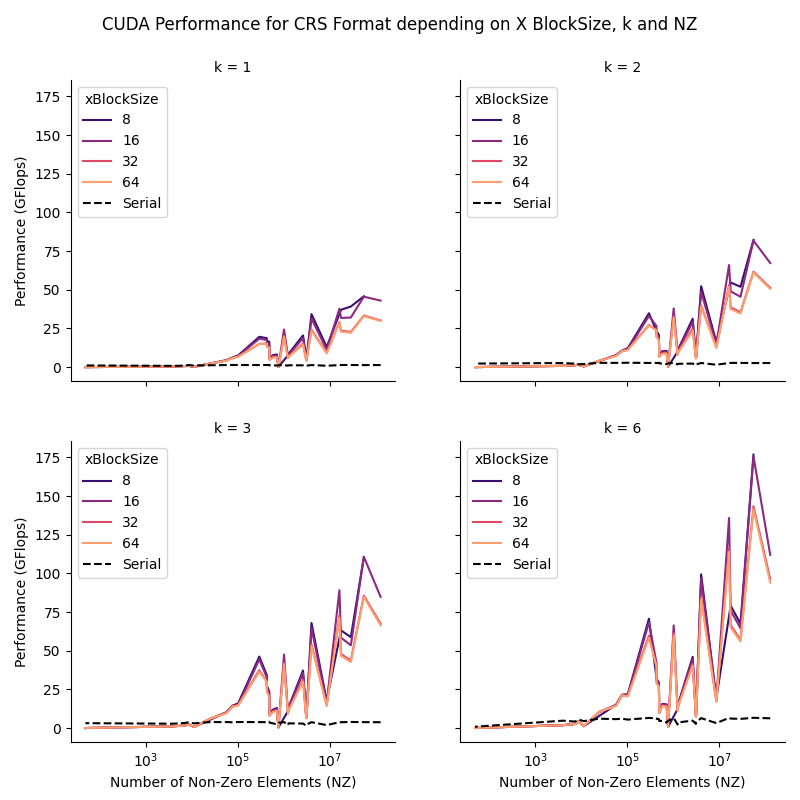
\includegraphics[width=0.6\textwidth]{../results/images/CUDA_xBlockSize_CRS.png}
    \caption{CUDA Performance for CRS Format depending on X BlockSize}
    \label{fig:cudaxblocksizecrs}
\end{figure}

\begin{figure}[H]
    \centering
    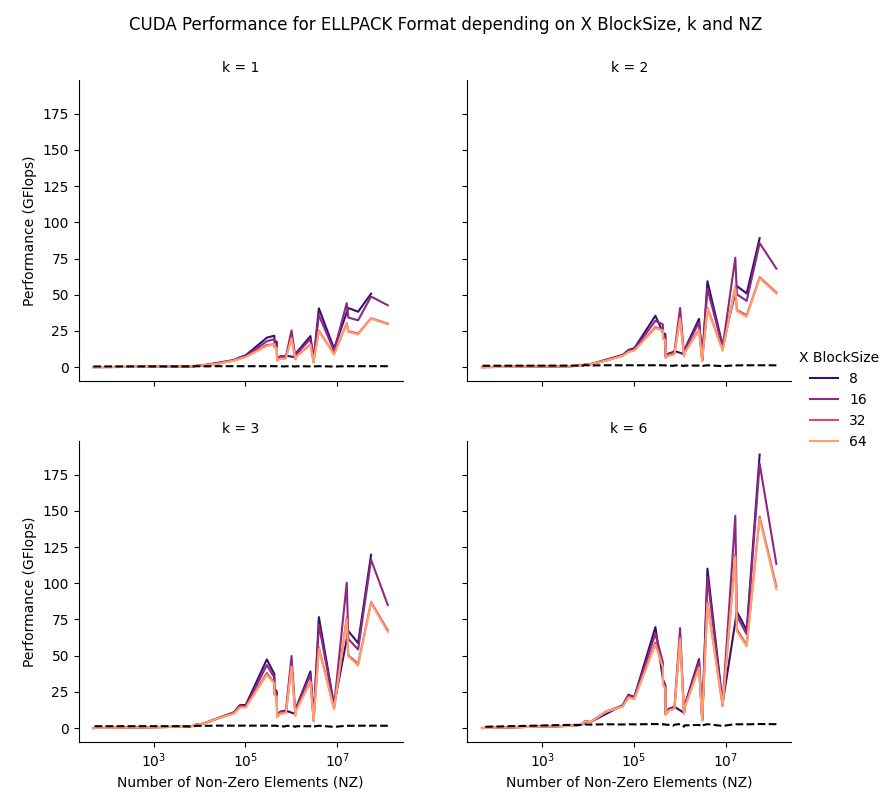
\includegraphics[width=0.6\textwidth]{../results/images/CUDA_xBlockSize_ELLPACK.png}
    \caption{CUDA Performance for ELLPACK Format depending on X BlockSize}
    \label{fig:cudaxblocksizeellpack}
\end{figure}

\subsubsection{Y Block Size Analysis}

\begin{figure}[H]
    \centering
    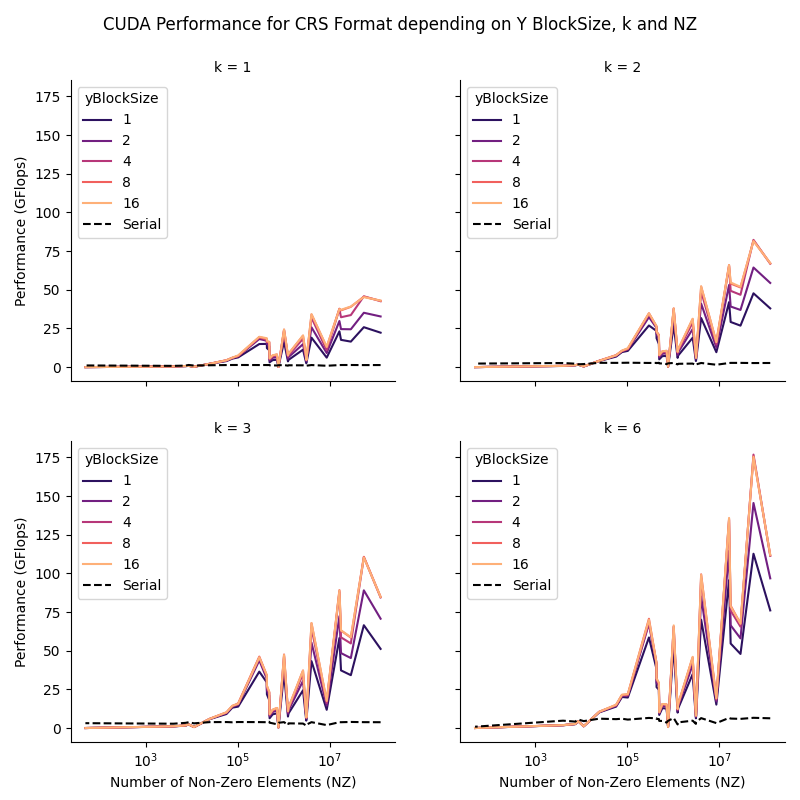
\includegraphics[width=0.6\textwidth]{../results/images/CUDA_yBlockSize_CRS.png}
    \caption{CUDA Performance for CRS Format depending on Y BlockSize}
    \label{fig:cudayblocksizecrs}
\end{figure}

\begin{figure}[H]
    \centering
    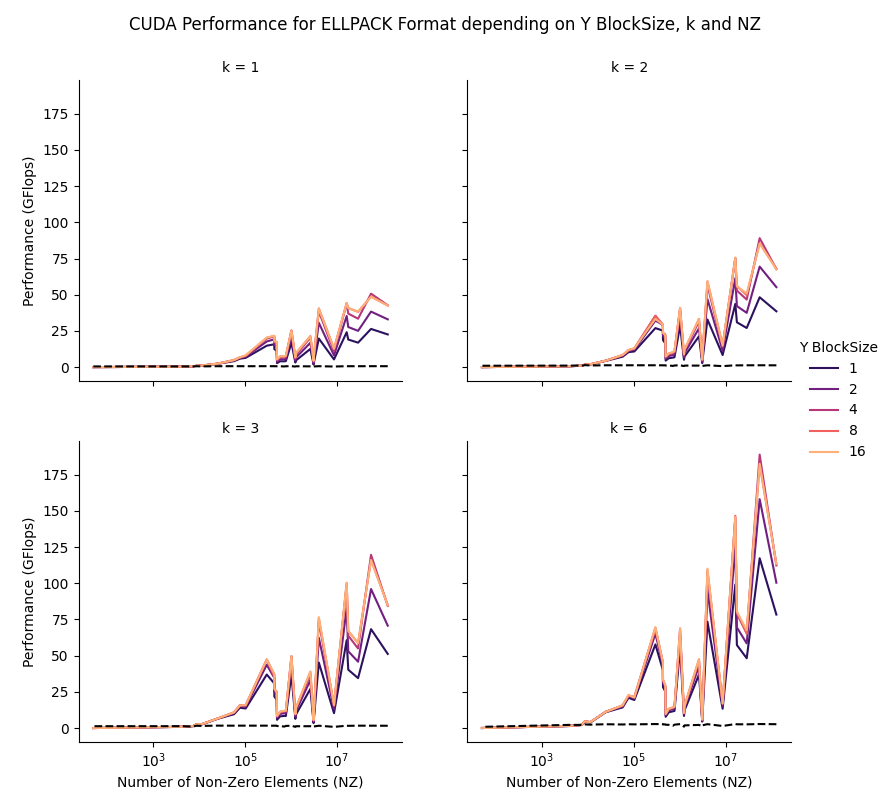
\includegraphics[width=0.6\textwidth]{../results/images/CUDA_yBlockSize_ELLPACK.png}
    \caption{CUDA Performance for ELLPACK Format depending on Y BlockSize}
    \label{fig:cudayblocksizeellpack}
\end{figure}

\subsubsection{Performance Comparison}

\begin{figure}[H]
    \centering
    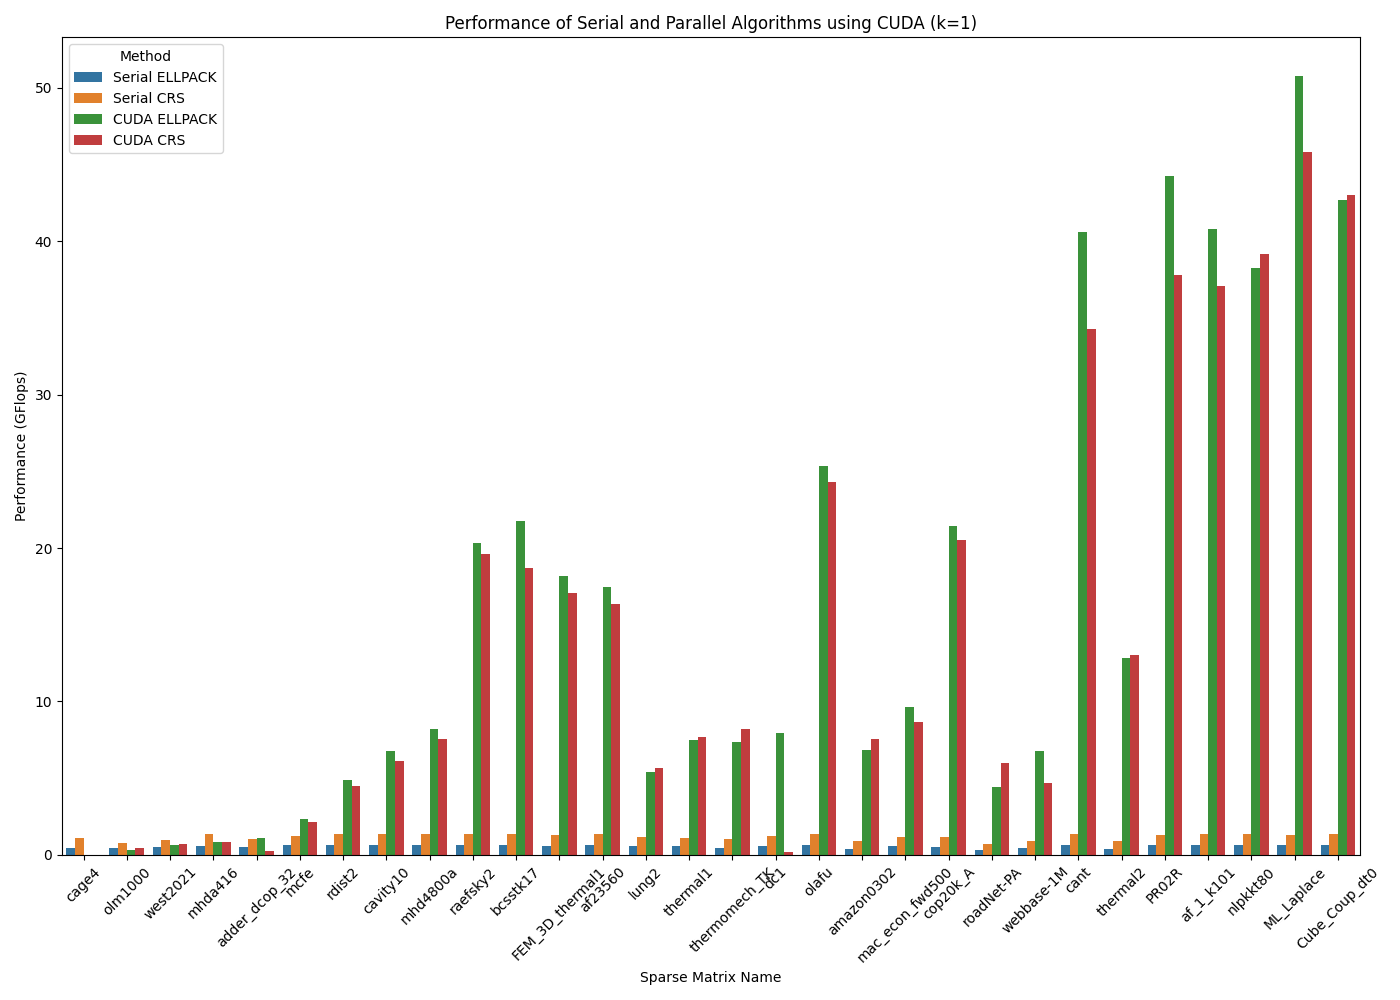
\includegraphics[width=0.9\textwidth]{../results/images/CUDA_Performance_k1.png}
    \caption{Performance of Serial and Parallel Algorithms using CUDA for $k=1$}
    \label{fig:cuda-performance-k1}
\end{figure}

\begin{figure}[H]
    \centering
    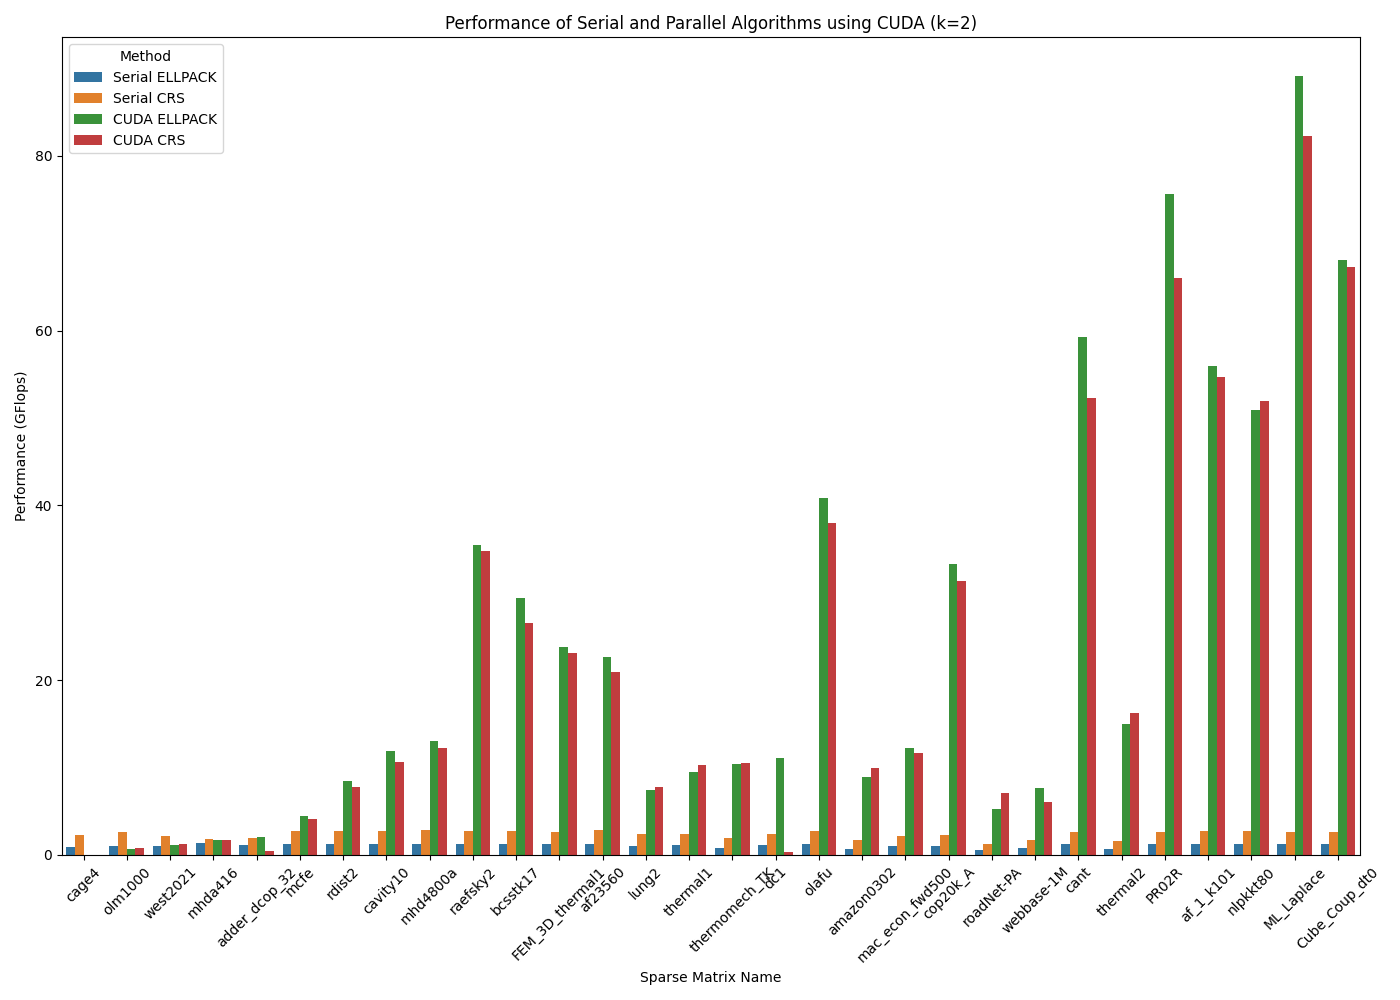
\includegraphics[width=0.9\textwidth]{../results/images/CUDA_Performance_k2.png}
    \caption{Performance of Serial and Parallel Algorithms using CUDA for $k=2$}
    \label{fig:cuda-performance-k2}
\end{figure}

\begin{figure}[H]
    \centering
    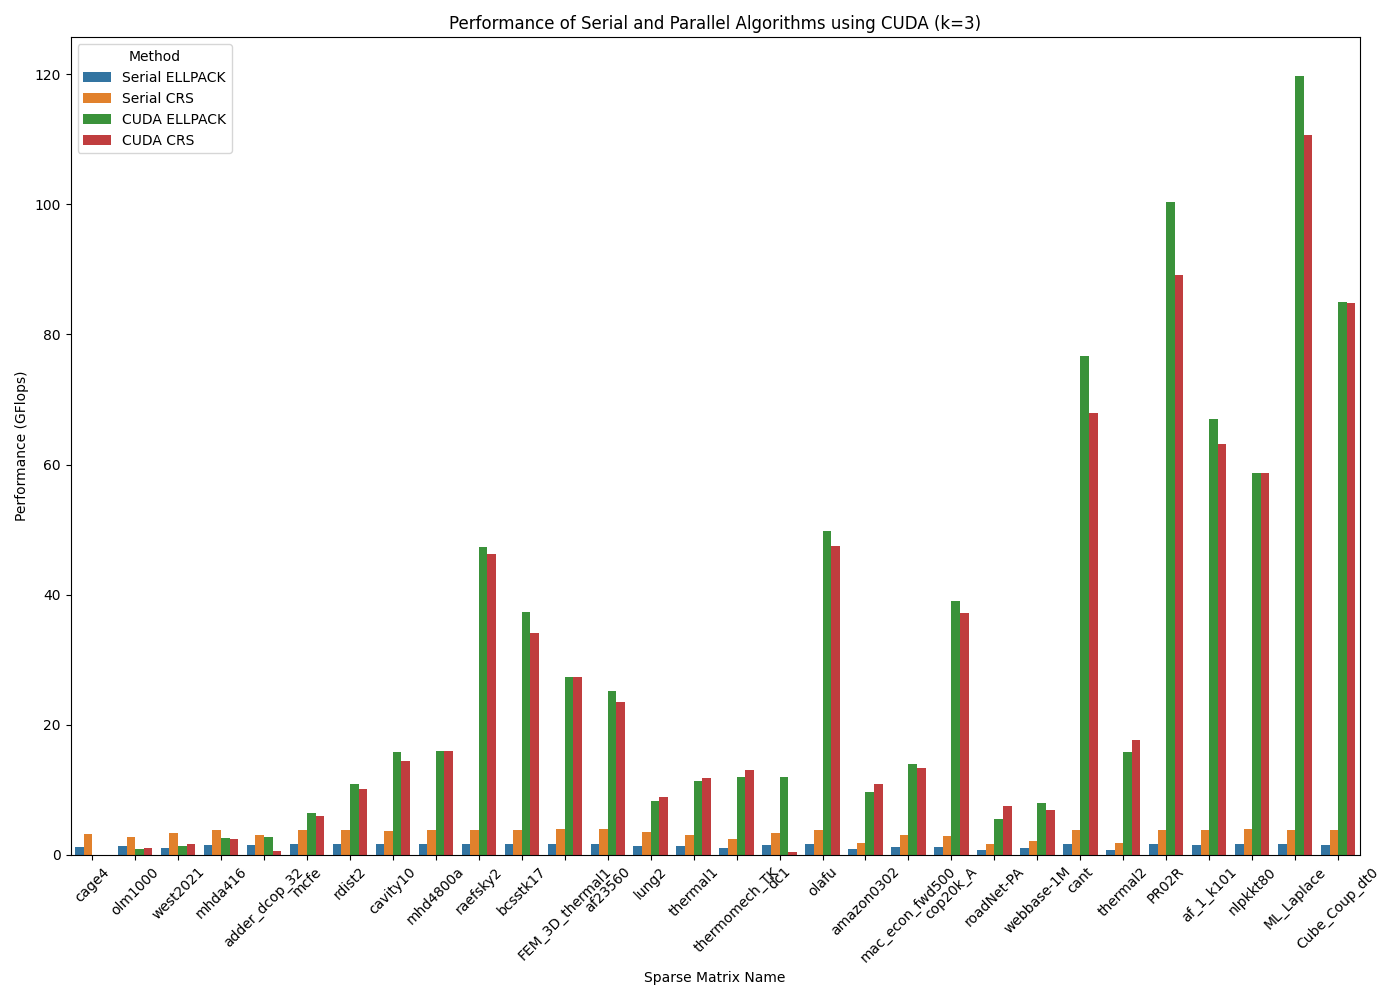
\includegraphics[width=0.9\textwidth]{../results/images/CUDA_Performance_k3.png}
    \caption{Performance of Serial and Parallel Algorithms using CUDA for $k=3$}
    \label{fig:cuda-performance-k3}
\end{figure}

\begin{figure}[H]
    \centering
    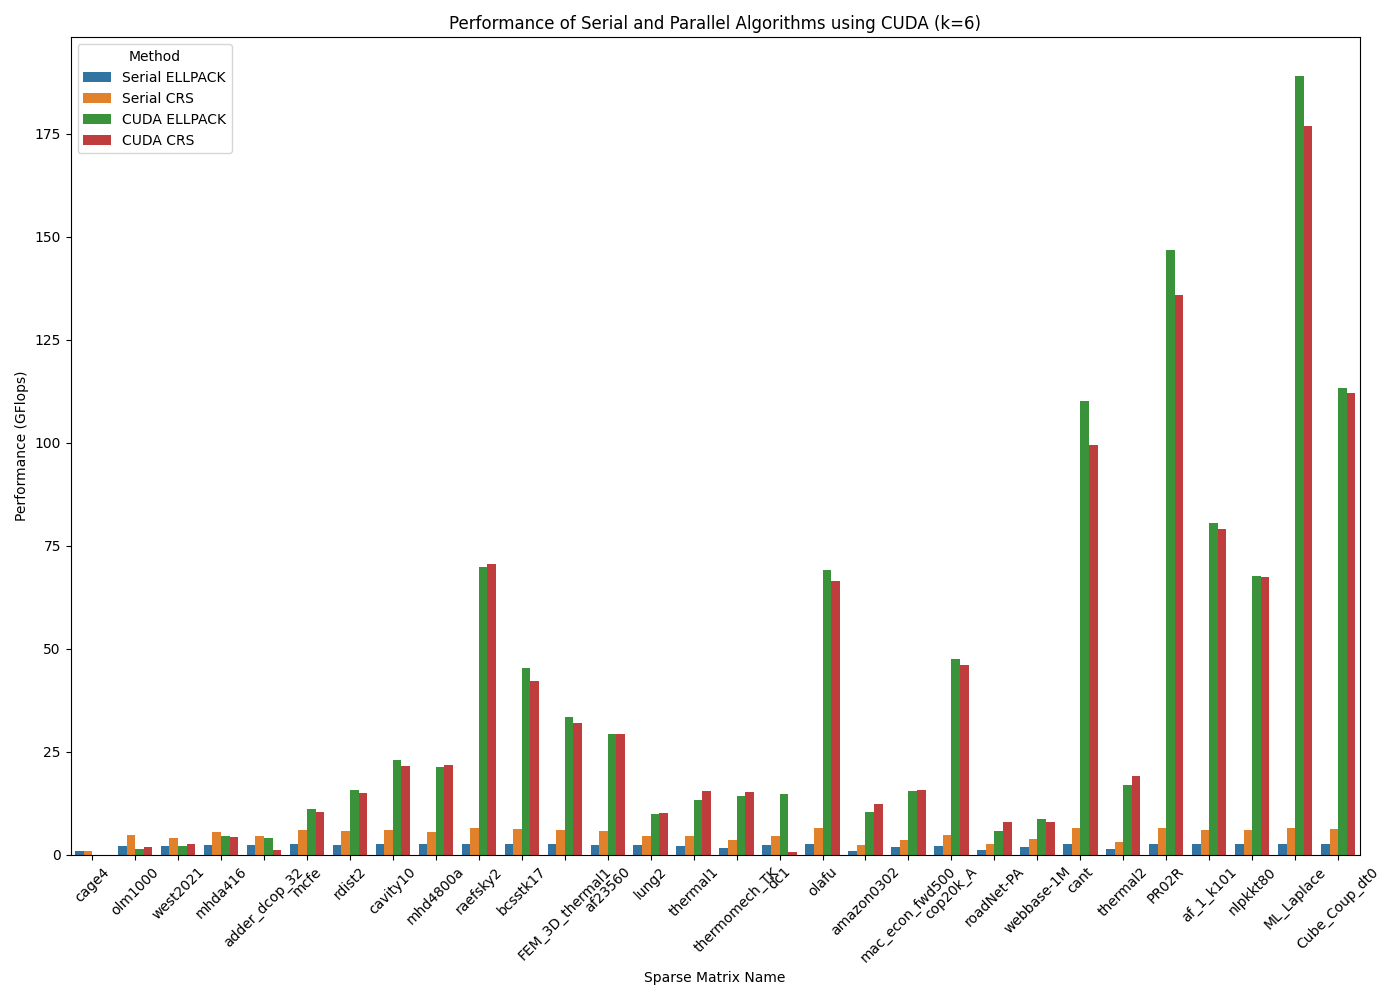
\includegraphics[width=0.9\textwidth]{../results/images/CUDA_Performance_k6.png}
    \caption{Performance of Serial and Parallel Algorithms using CUDA for $k=6$}
    \label{fig:cuda-performance-k6}
\end{figure}

\newpage
%TC:ignore 
\begin{longtable}{lcccr}
    \caption{CRS vs ELLPACK using CUDA}                                                              \\
    \label{tab:crsvsellpackcuda}                                                                     \\
    \toprule
    \textbf{Matrix}   & \textbf{CRS} & \textbf{ELLPACK} & \textbf{Best Structure} & \textbf{Speedup} \\
    \midrule
    \endfirsthead
    \toprule
    \textbf{Matrix}   & \textbf{CRS} & \textbf{ELLPACK} & \textbf{Best Structure} & \textbf{Speedup} \\
    \midrule
    \endhead
    \bottomrule
    \endfoot
    amazon0302        & 12.3120      & 10.4822          & CRS                     & 5.252515         \\
    cage4             & 0.033586     & 0.031649         & CRS                     & 0.038533         \\
    lung2             & 10.2714      & 9.81548          & CRS                     & 2.216157         \\
    mac\_econ\_fwd500 & 15.6609      & 15.4014          & CRS                     & 4.250389         \\
    mhd4800a          & 21.9362      & 21.4274          & CRS                     & 4.007095         \\
    olm1000           & 1.89504      & 1.48348          & CRS                     & 0.396840         \\
    raefsky2          & 70.6624      & 69.7615          & CRS                     & 10.778230        \\
    roadNet-PA        & 8.07317      & 5.84257          & CRS                     & 2.966768         \\
    thermal1          & 15.5753      & 13.318           & CRS                     & 3.386097         \\
    thermal2          & 19.2541      & 17.0523          & CRS                     & 6.004222         \\
    thermomech\_TK    & 15.3241      & 14.2953          & CRS                     & 4.305889         \\
    west2021          & 2.66929      & 2.26954          & CRS                     & 0.637915         \\
    Cube\_Coup\_dt0   & 111.963      & 113.348          & ELLPACK                 & 17.953161        \\
    FEM\_3D\_thermal1 & 32.0555      & 33.4671          & ELLPACK                 & 5.634524         \\
    ML\_Laplace       & 176.774      & 188.886          & ELLPACK                 & 28.493590        \\
    PR02R             & 135.828      & 146.651          & ELLPACK                 & 22.294501        \\
    adder\_dcop\_32   & 1.20824      & 4.12316          & ELLPACK                 & 0.920089         \\
    af23560           & 29.2923      & 29.4083          & ELLPACK                 & 5.066518         \\
    af\_1\_k101       & 79.1365      & 80.4176          & ELLPACK                 & 13.098161        \\
    bcsstk17          & 42.2982      & 45.3715          & ELLPACK                 & 7.251562         \\
    cant              & 99.3766      & 110.127          & ELLPACK                 & 17.154513        \\
    cavity10          & 21.571       & 23.0165          & ELLPACK                 & 3.815625         \\
    cop20k\_A         & 46.062       & 47.6264          & ELLPACK                 & 9.980867         \\
    dc1               & 0.733577     & 14.7532          & ELLPACK                 & 3.147779         \\
    mcfe              & 10.5186      & 11.2408          & ELLPACK                 & 1.852130         \\
    mhda416           & 4.46372      & 4.6875           & ELLPACK                 & 0.848498         \\
    nlpkkt80          & 67.4344      & 67.5926          & ELLPACK                 & 11.394303        \\
    olafu             & 66.3819      & 69.052           & ELLPACK                 & 10.654512        \\
    rdist2            & 15.0779      & 15.7503          & ELLPACK                 & 2.733008         \\
    webbase-1M        & 8.04237      & 8.68042          & ELLPACK                 & 2.314507         \\
\end{longtable}
%TC:endignore

The results of parallelizing the CRS and ELLPACK algorithms with CUDA show a
strong preference for the CRS format on certain matrices (such as
\textit{amazon0302}, \textit{lung2}, and \textit{thermal1}), attributable to
better sparsity management and memory access patterns optimized for GPUs. In
contrast, ELLPACK shows superior performance for matrices with regular
structures, such as \textit{Cube\_Coup\_dt0} and \textit{ML\_Laplace}, due to
more uniform memory access.

The variability of the speed-up factor between matrices highlights the
importance of the specific structure of the matrix in the relative efficiency
of CRS and ELLPACK under CUDA. In particular, symmetric and dense arrays tend
to favour ELLPACK, highlighting the significant role of density and symmetry in
the performance of the formats.

\subsection{Overall Performance Comparison}
\begin{figure}[H]
    \centering
    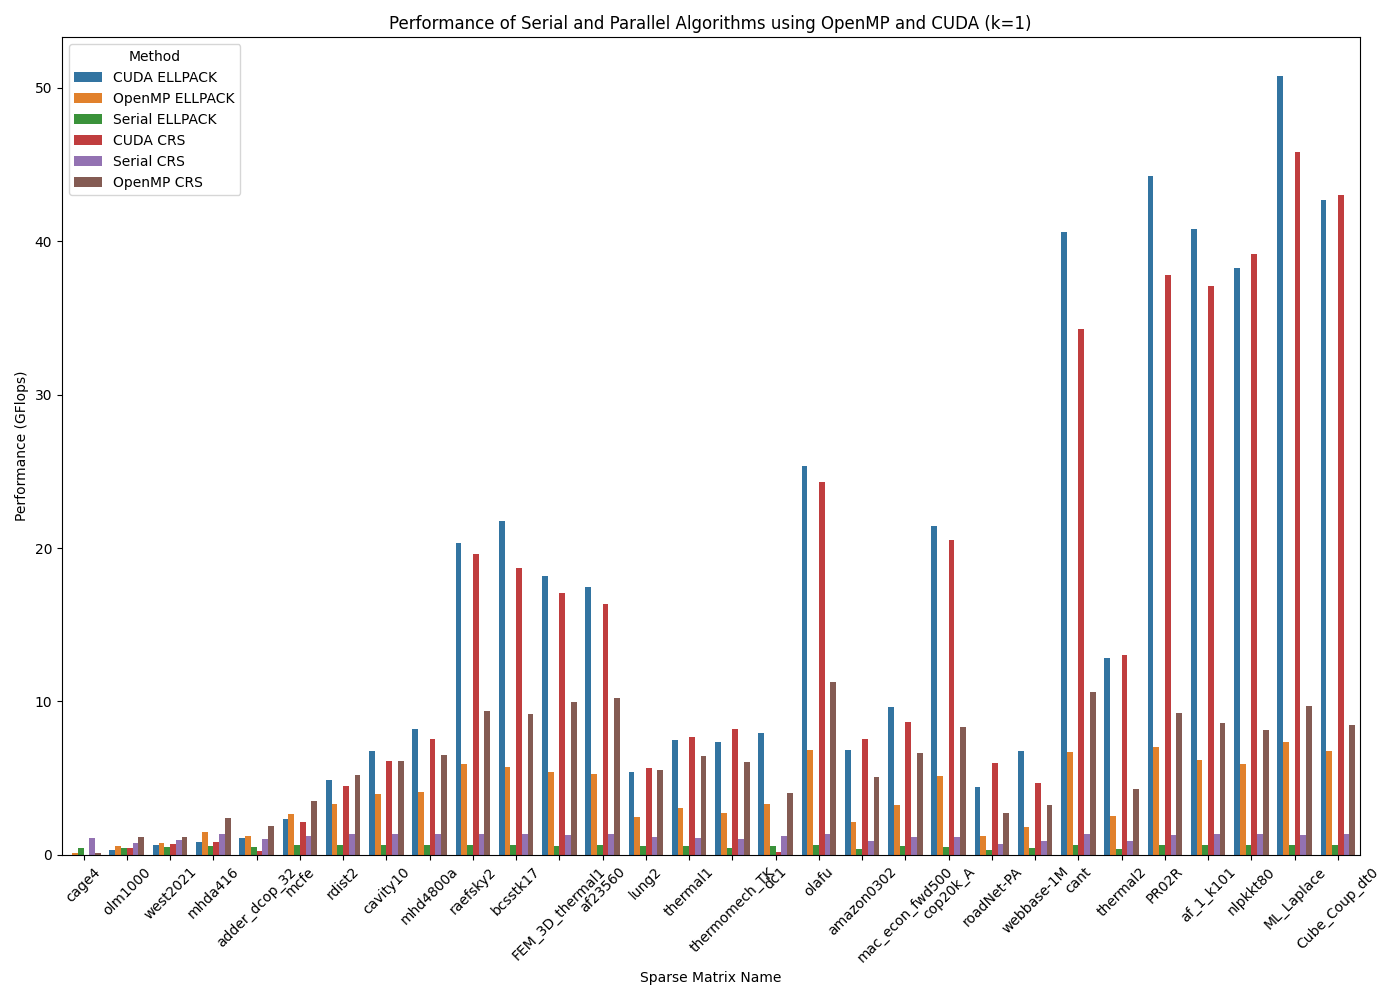
\includegraphics[width=0.8\textwidth]{../results/images/OpenMP_vs_CUDA_Performance_k1.png}
    \caption{OpenMP vs CUDA Performance for $k=1$}
    \label{fig:openmp-cuda-performance-k1}
\end{figure}

\begin{figure}[H]
    \centering
    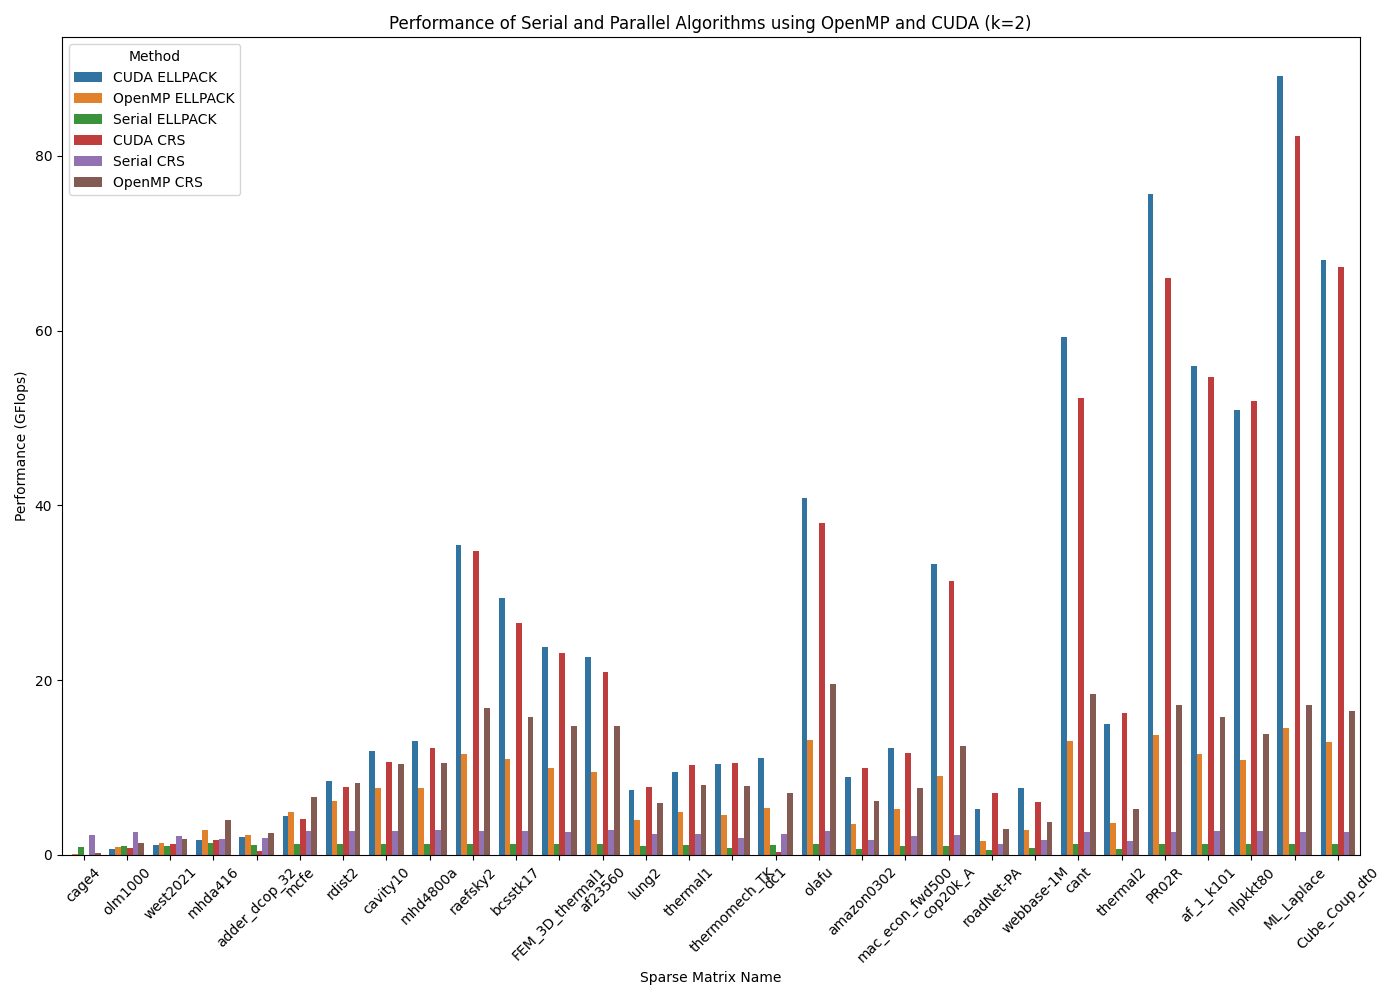
\includegraphics[width=0.8\textwidth]{../results/images/OpenMP_vs_CUDA_Performance_k2.png}
    \caption{OpenMP vs CUDA Performance for $k=2$}
    \label{fig:openmp-cuda-performance-k2}
\end{figure}

\begin{figure}[H]
    \centering
    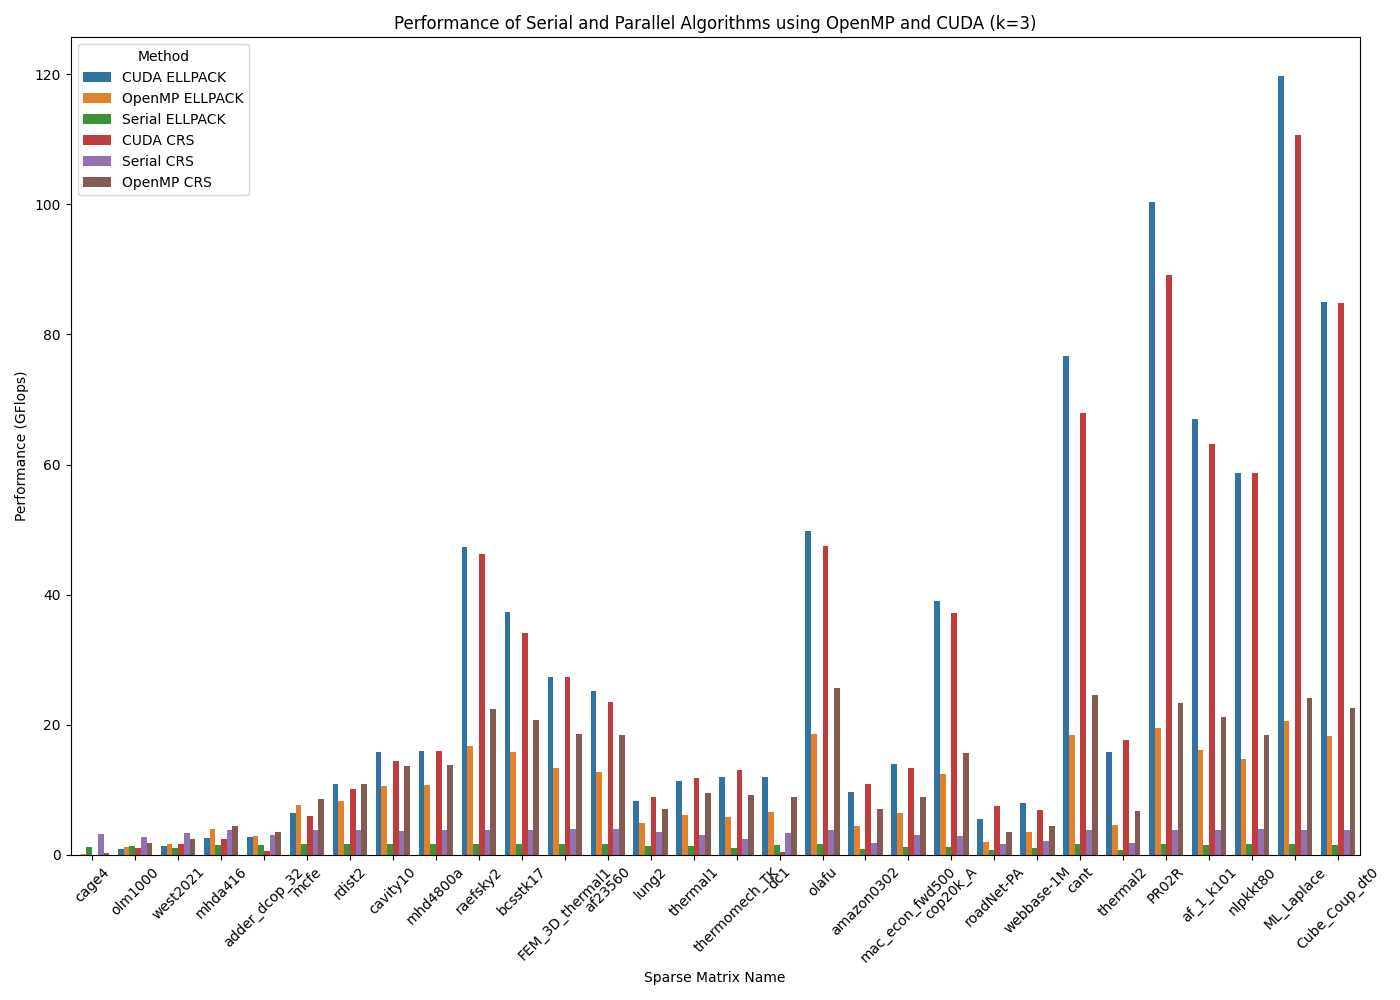
\includegraphics[width=0.7\textwidth]{../results/images/OpenMP_vs_CUDA_Performance_k3.png}
    \caption{OpenMP vs CUDA Performance for $k=3$}
    \label{fig:openmp-cuda-performance-k3}
\end{figure}

\begin{figure}[H]
    \centering
    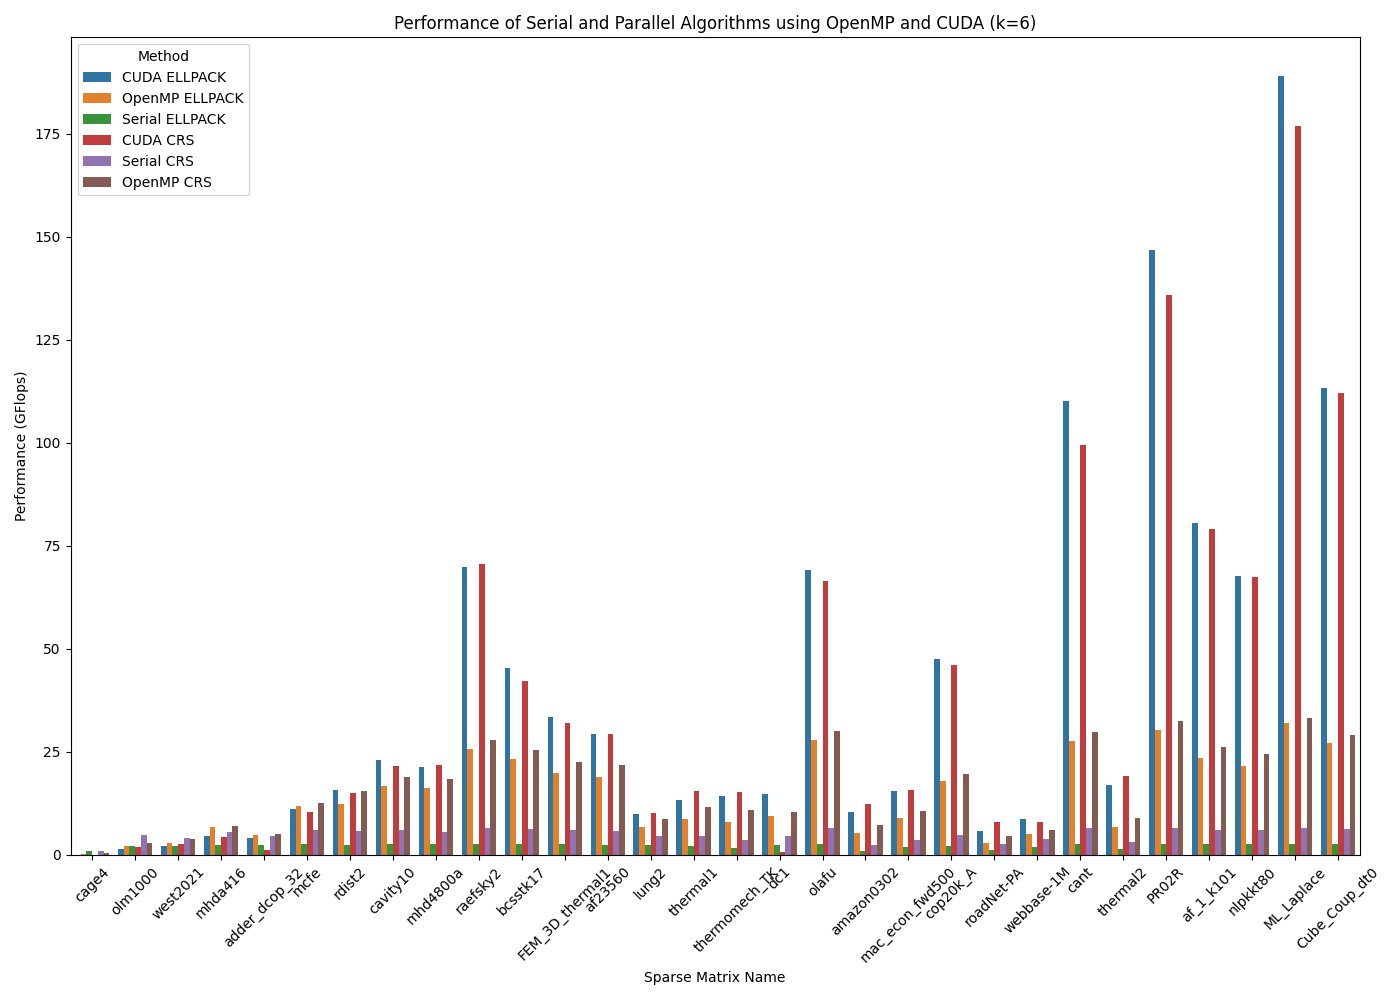
\includegraphics[width=0.7\textwidth]{../results/images/OpenMP_vs_CUDA_Performance_k6.png}
    \caption{OpenMP vs CUDA Performance for $k=6$}
    \label{fig:openmp-cuda-performance-k6}
\end{figure}

%TC:ignore 
\begin{longtable}{lccccr}
    \caption{Overall Performance Comparison}                                                                          \\
    \label{tab:overallperformance}                                                                                    \\
    \toprule
    \textbf{Matrix}   & \textbf{Best Performance} & \textbf{Best Structure} & \textbf{Best Method} & \textbf{Speedup} \\
    \midrule
    \endfirsthead
    \toprule
    \textbf{Matrix}   & \textbf{Best Performance} & \textbf{Best Structure} & \textbf{Best Method} & \textbf{Speedup} \\
    \midrule
    \endhead
    \bottomrule
    \endfoot
    amazon0302        & 12.3120                   & CRS                     & CUDA                 & 5.252515         \\
    lung2             & 10.2714                   & CRS                     & CUDA                 & 2.216157         \\
    mac\_econ\_fwd500 & 15.6609                   & CRS                     & CUDA                 & 4.250389         \\
    mhd4800a          & 21.9362                   & CRS                     & CUDA                 & 4.007095         \\
    raefsky2          & 70.6624                   & CRS                     & CUDA                 & 10.778230        \\
    roadNet-PA        & 8.07317                   & CRS                     & CUDA                 & 2.966768         \\
    thermal1          & 15.5753                   & CRS                     & CUDA                 & 3.386097         \\
    thermal2          & 19.2541                   & CRS                     & CUDA                 & 6.004222         \\
    thermomech\_TK    & 15.3241                   & CRS                     & CUDA                 & 4.305889         \\
    Cube\_Coup\_dt0   & 113.348                   & ELLPACK                 & CUDA                 & 17.953161        \\
    FEM\_3D\_thermal1 & 33.4671                   & ELLPACK                 & CUDA                 & 5.634524         \\
    ML\_Laplace       & 188.886                   & ELLPACK                 & CUDA                 & 28.493590        \\
    PR02R             & 146.651                   & ELLPACK                 & CUDA                 & 22.294501        \\
    af23560           & 29.4083                   & ELLPACK                 & CUDA                 & 5.066518         \\
    af\_1\_k101       & 80.4176                   & ELLPACK                 & CUDA                 & 13.098161        \\
    bcsstk17          & 45.3715                   & ELLPACK                 & CUDA                 & 7.251562         \\
    cant              & 110.127                   & ELLPACK                 & CUDA                 & 17.154513        \\
    cavity10          & 23.0165                   & ELLPACK                 & CUDA                 & 3.815625         \\
    cop20k\_A         & 47.6264                   & ELLPACK                 & CUDA                 & 9.980867         \\
    dc1               & 14.7532                   & ELLPACK                 & CUDA                 & 3.147779         \\
    nlpkkt80          & 67.5926                   & ELLPACK                 & CUDA                 & 11.394303        \\
    olafu             & 69.0520                   & ELLPACK                 & CUDA                 & 10.654512        \\
    rdist2            & 15.7503                   & ELLPACK                 & CUDA                 & 2.733008         \\
    webbase-1M        & 8.68042                   & ELLPACK                 & CUDA                 & 2.314507         \\
    adder\_dcop\_32   & 5.12204                   & CRS                     & OpenMP               & 1.142991         \\
    mcfe              & 12.6097                   & CRS                     & OpenMP               & 2.077682         \\
    mhda416           & 7.06099                   & CRS                     & OpenMP               & 1.278130         \\
    cage4             & 0.871628                  & CRS                     & Serial               & 1.000000         \\
    olm1000           & 4.77532                   & CRS                     & Serial               & 1.000000         \\
    west2021          & 4.1844                    & CRS                     & Serial               & 1.000000         \\
\end{longtable}
%TC:endignore

Exceptionally high performance is observed for certain matrices under CUDA,
such as \textit{Cube\_Coup\_dt0} and \textit{ML\_Laplace}, revealing the match
between certain data structures and GPU optimisation. On the other hand, OpenMP
shows a moderate advantage for specific matrices, such as
\textit{adder\_dcop\_32} and \textit{mcfe}, offering a significant performance
improvement without the need for specialised hardware, thanks to
parallelization on shared memory architectures.

However, matrices of small size or with characteristics less favourable to
parallelization, such as \textit{cage4}, \textit{olm1000}, and
\textit{west2021}, show no significant improvement with OpenMP or CUDA,
indicating that for some cases sequential execution remains the most suitable
method.

These observations lead to the conclusion that the choice between CRS and
ELLPACK formats, as well as the decision to use sequential execution, OpenMP or
CUDA, should be informed by the specific properties of the matrices in
question. Optimisation of the calculation parameters and careful evaluation of
the data characteristics are essential to maximise the efficiency of operations
on hollow matrices.

\chapter{Conclusion}

In summary, this report explored the performance of the CSR and ELLPACK formats
for dense vector multiplication of hollow matrices using the OpenMP and CUDA
parallel programming paradigms. The results show a marked preference for the
CSR format when parallelized with OpenMP, which is probably due to more
efficient memory management and optimal task distribution between threads. On
the other hand, CUDA performance is strongly influenced by the sparsity and
structural regularity of matrices, with symmetric and dense matrices seemingly
favouring the ELLPACK format.

The benefits of using CUDA on GPU architectures have been demonstrated,
particularly for arrays that align well with memory access models optimised for
these devices. However, it is clear that the benefits of parallelization with
CUDA or OpenMP are closely related to the specific characteristics of the
arrays in question, and that a sequential approach may be preferable for small
arrays or those with patterns less conducive to parallelization.

These findings underline the importance of a thorough analysis of data
structures and computational parameters to maximise the efficiency of
operations on hollow matrices. Ultimately, the choice between CSR and ELLPACK
formats, as well as the decision to use sequential execution, OpenMP or CUDA,
must be informed by the specific properties of the matrices. Such a nuanced
understanding will further optimise the performance of the scientific and
engineering applications that depend on these intensive computations.

\bibliographystyle{CranfieldNumbered}
\bibliography{CUCitations}

%TC:ignore 
\appendix
\chapter{Documentation}

\begin{subappendices}
    \section{Project tree}
    \begin{lstlisting}[breaklines=true, basicstyle=\small]
    Source Code/
        CRS/
            matrixMultivectorProductCRS.cpp
            matrixMultivectorProductCRS.h
            matrixMultivectorProductCRSCUDA.cu
            matrixMultivectorProductCRSCUDA.h
            matrixMultivectorProductCRSOpenMP.cpp
            matrixMultivectorProductCRSOpenMP.h
        ELLPACK/
            matrixMultivectorProductELLPACK.cpp
            matrixMultivectorProductELLPACK.h
            matrixMultivectorProductELLPACKCUDA.cu
            matrixMultivectorProductELLPACKCUDA.h
            matrixMultivectorProductELLPACKOpenMP.cpp
            matrixMultivectorProductELLPACKOpenMP.h
        scripts/
            cuda.sub
            openMP.sub
            parseCudaResults.sh
            parseOpenMPResults.sh
        cudaUtils.cuh
        makefile
        MatrixDefinitions.h
        runCuda.cpp
        runOpenMP.cpp
        utils.h
        utils.cpp
    results/
        images/
        CUDA.csv
        CUDA.ipynb
        OpenMP.csv
        OpenMP.ipynb
    \end{lstlisting}

    \section{Getting Started}
    To run the program, follow these steps:
    \begin{enumerate}
        \itemindent=17.87pt
        \item Install the required compilers and libraries:
              \begin{itemize}
                  \item \textbf{OpenMP:} Install the GNU Compiler Collection (GCC) and OpenMP~\cite{GCC}.
                  \item \textbf{CUDA:} Install the NVIDIA CUDA Toolkit~\cite{CUDA}.
              \end{itemize}
        \item Compile the files using the following command: \texttt{make all}.
        \item Run the programs:
              \begin{itemize}
                  \item \textbf{OpenMP:} \texttt{./runOpenMP.o}
                  \item  \textbf{CUDA:} \texttt{./runCuda.o}
              \end{itemize}
    \end{enumerate}

    \section{Methods Overview}
    \subsection{Utils.h}
    \subsubsection{convertCRStoELLPACK}
    \textbf{Description:} Read a sparse matrix from a Matrix Market file.\\

    \textbf{Parameters:}
    \begin{itemize}
        \item \texttt{SparseMatrixCRS \&crsMatrix}: The CRS matrix to convert.
        \item \texttt{SparseMatrixELLPACK \&ellpackMatrix}: The ELLPACK matrix to convert to.
    \end{itemize}

    \subsubsection{areMatricesEqual}
    \textbf{Description:} Compares two matrices for equality within a specified tolerance.\\

    \textbf{Parameters:}
    \begin{itemize}
        \item \texttt{FatVector \&mat1}: First matrix.
        \item \texttt{FatVector \&mat2}: Second matrix.
        \item \texttt{double tolerance}: Tolerance for comparison.
    \end{itemize}

    \textbf{Returns:} \texttt{bool}: True if matrices are equal within the tolerance, false otherwise.

    \subsubsection{readMatrixMarketFile}
    \textbf{Description:} Reads a matrix from a Matrix Market file into a sparse matrix format.\\

    \textbf{Parameters:}
    \begin{itemize}
        \item \texttt{std::string \&filename}: Name of the Matrix Market file.
        \item \texttt{SparseMatrixCRS \&matrix}: Sparse matrix to read into.
    \end{itemize}

    \subsubsection{generateLargeFatVector}
    \textbf{Description:} Generates a random Fat Vector with specified dimensions.\\

    \textbf{Parameters:}
    \begin{itemize}
        \item \texttt{FatVector \&fatVector}: Fat vector to generate.
        \item \texttt{int n}: Number of rows.
        \item \texttt{int k}: Number of columns.
    \end{itemize}

    \subsection{matrixMultivectorProductCRS.h}
    \subsubsection{matrixMultivectorProductCRS}
    \textbf{Description:} Perform the matrix-vector multiplication in the CRS format.\\

    \textbf{Parameters:}
    \begin{itemize}
        \item \texttt{SparseMatrixCRS \&sparseMatrix}: Sparse matrix in CRS format.
        \item \texttt{FatVector \&fatVector}: Fat vector.
        \item \texttt{FatVector \&result}: Result of the multiplication.
        \item \texttt{int testNumber}: Number of iterations for the performance measurement
    \end{itemize}

    \subsection{matrixMultivectorProductCRSOpenMP.h}
    \subsubsection{matrixMultivectorProductCRSOpenMP}
    \textbf{Description:} Perform the matrix-vector multiplication in the CRS format using OpenMP\\

    \textbf{Parameters:}
    \begin{itemize}
        \item \texttt{SparseMatrixCRS \&sparseMatrix}: Sparse matrix in CRS format.
        \item \texttt{FatVector \&fatVector}: Fat vector.
        \item \texttt{FatVector \&result}: Result of the multiplication.
        \item \texttt{int testNumber}: Number of iterations for the performance measurement
        \item \texttt{int numThreads}: Number of threads to use.
        \item \texttt{int chunkSize}: Chunk size for the parallelization.
    \end{itemize}

    \subsection{matrixMultivectorProductCRSCUDA.h}
    \subsubsection{matrixMultivectorProductCRSCUDA}
    \textbf{Description:} Perform the matrix-vector multiplication in the CRS format using CUDA\\

    \textbf{Parameters:}
    \begin{itemize}
        \item \texttt{SparseMatrixCRS \&sparseMatrix}: Sparse matrix in CRS format.
        \item \texttt{FatVector \&fatVector}: Fat vector.
        \item \texttt{FatVector \&result}: Result of the multiplication.
        \item \texttt{int testNumber}: Number of iterations for the performance measurement
        \item \texttt{int xBlockSize}: X block size for the parallelization.
        \item \texttt{int yBlockSize}: Y block size for the parallelization.
    \end{itemize}

    \subsection{matrixMultivectorProductELLPACK.h}
    \subsubsection{matrixMultivectorProductELLPACK}
    \textbf{Description:} Perform the matrix-vector multiplication in the ELLPACK format.\\

    \textbf{Parameters:}
    \begin{itemize}
        \item \texttt{SparseMatrixELLPACK \&sparseMatrix}: Sparse matrix in ELLPACK format.
        \item \texttt{FatVector \&fatVector}: Fat vector.
        \item \texttt{FatVector \&result}: Result of the multiplication.
        \item \texttt{int testNumber}: Number of iterations for the performance measurement
    \end{itemize}

    \subsection{matrixMultivectorProductELLPACKOpenMP.h}
    \subsubsection{matrixMultivectorProductELLPACKOpenMP}
    \textbf{Description:} Perform the matrix-vector multiplication in the ELLPACK format using OpenMP\\

    \textbf{Parameters:}
    \begin{itemize}
        \item \texttt{SparseMatrixELLPACK \&sparseMatrix}: Sparse matrix in ELLPACK format.
        \item \texttt{FatVector \&fatVector}: Fat vector.
        \item \texttt{FatVector \&result}: Result of the multiplication.
        \item \texttt{int testNumber}: Number of iterations for the performance measurement
        \item \texttt{int numThreads}: Number of threads to use.
        \item \texttt{int chunkSize}: Chunk size for the parallelization.
    \end{itemize}

    \subsection{matrixMultivectorProductELLPACKCUDA.h}
    \subsubsection{matrixMultivectorProductELLPACKCUDA}
    \textbf{Description:} Perform the matrix-vector multiplication in the ELLPACK format using CUDA\\

    \textbf{Parameters:}
    \begin{itemize}
        \item \texttt{SparseMatrixELLPACK \&sparseMatrix}: Sparse matrix in ELLPACK format.
        \item \texttt{FatVector \&fatVector}: Fat vector.
        \item \texttt{FatVector \&result}: Result of the multiplication.
        \item \texttt{int testNumber}: Number of iterations for the performance measurement
        \item \texttt{int xBlockSize}: X block size for the parallelization.
        \item \texttt{int yBlockSize}: Y block size for the parallelization.
    \end{itemize}


\end{subappendices}

\chapter{Source Codes}
\begin{subappendices}
    \section{Data Structures}\label{appendix:data-structures}
    Data stuctures of the sparse matrix in the CRS and ELLPACK formats, as well as
    the FatVector structure. \lstinputlisting[style=cstyle]{../Source
        Code/MatrixDefinitions.h}

    \newpage
    \section{Sequential Algorithm}\label{appendix:sequential}
    \subsection{CRS Format}\label{appendix:crs-sequential}
    \lstinputlisting[style=cstyle]{../Source Code/CRS/matrixMultivectorProductCRS.cpp}

    \subsection{ELLPACK Format}\label{appendix:ellpack-sequential}
    \lstinputlisting[style=cstyle]{../Source Code/ELLPACK/matrixMultivectorProductELLPACK.cpp}

    \newpage
    \section{OpenMP Parallel Algorithm}\label{appendix:openmp}
    \subsection{CRS Format}\label{appendix:crs-openmp}
    \lstinputlisting[style=cstyle]{../Source Code/CRS/matrixMultivectorProductCRSOpenMP.cpp}

    \subsection{ELLPACK Format}\label{appendix:ellpack-openmp}
    \lstinputlisting[style=cstyle]{../Source Code/ELLPACK/matrixMultivectorProductELLPACKOpenMP.cpp}

    \newpage
    \section{CUDA Parallel Algorithm}\label{appendix:cuda}
    \subsection{CRS Format}\label{appendix:crs-cuda}
    \lstinputlisting[style=cstyle]{../Source Code/CRS/matrixMultivectorProductCRSCUDA.cu}

    \subsection{ELLPACK Format}\label{appendix:ellpack-cuda}
    \lstinputlisting[style=cstyle]{../Source Code/ELLPACK/matrixMultivectorProductELLPACKCUDA.cu}

    \newpage
    \section{Utilities}\label{appendix:utilities}
    \lstinputlisting[style=cstyle]{../Source Code/utils.cpp}

    \newpage
    \section{Main Program}\label{appendix:main}
    \subsection{OpenMP}\label{appendix:openmp-main}
    \lstinputlisting[style=cstyle]{../Source Code/runOpenMP.cpp}

    \subsection{CUDA}\label{appendix:cuda-main}
    \lstinputlisting[style=cstyle]{../Source Code/runCuda.cpp}

\end{subappendices}
%TC:endignore 

\end{document}

